% Aquí contendrán los métodos y procedimientos adoptados en el desarrollo del trabajo. Esta es una de las sesiones más importantes pues demuestra el poder científico que se utilizó para la investigación. Sin una buena metodología la investigación puede perder la validez. El investigador debe utilizar métodos o técnicas aceptadas por la comunidad científica en la búsqueda de probar sus hipótesis.

% La metodología elegida debe ser aquella que más se adecue a su objeto de estudio y al enfoque aplicado. Hay dos métodos principales: 1) cuantitativo, que es el uso de instrumental estadístico, de datos numéricos; y 2) cualitativo, que se caracteriza por la calificación de los datos recogidos, durante el análisis del problema.

% ENLACES VISTOS
% COURSERA: La Web Semántica: Herramientas para la publicación y extracción efectiva de información en la Web
% CURSO EN COURSERA INTERESANTE: https://es.coursera.org/learn/web-semantica?action=enroll
% http://www.fgcsic.es/lychnos/es_es/articulos/construyendo_una_web_semantica
% Libro Geospatial Semantic Web
% https://www.researchgate.net/publication/216537707_La_Web_semantica_y_las_tecnologias_del_lenguaje_humano
% http://www.bibliopos.es/Biblion-A2-Bibliografia-Documentacion/18ontologia-Web-Semantica.pdf

\chapter{Web Semántica}
\label{ch:web-semantinca}

\begin{quote}
  {\bf\textsc{Resumen:}} En este capítulo se presenta la Web Semántica como una extensión de la Web actual que nos ayuda a encontrar respuestas a preguntas en Internet haciendo uso de la información semántica contenida en la búsqueda, gracias a una información mejor definida. Los conocimientos que adquiramos a lo largo de este capítulo sirven como base para el posterior desarrollo del ejemplo práctico. De esta manera, dividiremos el capítulo en tres grandes apartados: el primero de ellos contextualiza y explica la Web Semántica, el segundo nos adentra en las capas de la arquitectura de la Web Semántica, y el tercero habla sobre aplicaciones y posibilidades futuras que presenta la Web Semántica.
\end{quote}

\section{Web Semántica}

A continuación, vamos a introducir la definición de Web Semántica, para ello es necesario realizar un breve estudio del arte sobre la Web actual, para así comprender su origen y contexto en el que nace.

\subsection{Conceptos Generales}

%% ANTECEDENTES
%% DEFINICIÓN DE WEB, CUANDO SE CREO, QUIEN LA CREO, COMO SURGIÓ

% https://disenowebakus.net/semantica-web.php
% tesis
La revolución informática, acaecida durante el siglo XX, llevó consigo la introducción de cambios severos en distintos aspectos de la sociedad. De entre todas estas transformaciones, fueron muchos los que vaticinaron un nuevo mundo, fundamentado principalmente por la aparición de la informática personal, en donde los seres humanos tendrían acceso a grandes repositorios de información \cite{semantica-web}. Este hecho trajo consigo el desarrollo, por parte del físico Tim Berners-Lee del CERN\footnote{El \href{https://home.cern}{CERN}, Organización Europea para la Investigación Nuclear, es uno de los centros de investigación científica más grandes y respetados del mundo ubicado en Suiza.}, de un sistema de vinculación y transferencia de documentos en red que acabaría convirtiéndose en la World Wide Web (WWW) o Red Global Mundial, actualmente conocida como la \textbf{Web} \cite{tesis}.\\
%.creada por Tim Berners-Lee en 1989 y presentada en el CERN\footnote{El \href{https://home.cern}{CERN}, Organización Europea para la Investigación Nuclear, es uno de los centros de investigación científica más grandes y respetados del mundo.} (Suiza) \cite{tesis}. \\

% https://www.researchgate.net/publication/216537707_La_Web_semantica_y_las_tecnologias_del_lenguaje_humano
% COURSERA: La Web Semántica: Herramientas para la publicación y extracción efectiva de información en la Web
A lo largo de la literatura, muchos son los autores que han definido la Web Semántica como la Web del futuro. Sin embargo, para poder comprenderla es necesario entender bien cuál es la Web actual \cite{researchgate}. En términos generales, la Web actual es una red informática compuesta por multitud de documentos \cite{coursera}. Estos documentos son básicamente páginas Web que hacen uso del lenguaje natural para expresar sus contenidos (texto, imágenes, audios, enlaces) y de etiquetas HTML (\textit{HyperText Markup Language}) para su interpretación en los navegadores Web (Figura \ref{html}). 

% https://fjph32html.wordpress.com/2015/03/08/leccion-3-estructura-basica-en-html/
\begin{figure}[H]
	\centering
	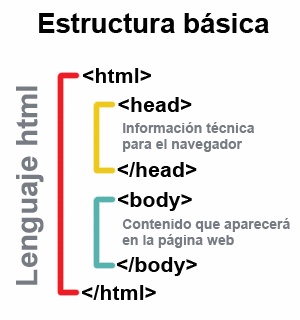
\includegraphics[height=5.6cm]{imagenes/capitulo3/estructurabasica} 
	\caption{Ejemplo de la estructura HTML \cite{imagen-html}}
	\label{html}
\end{figure}

En la figura \ref{fig:web} se puede apreciar como ha evolucionado la Web desde sus inicios hasta la Web Semántica (para saber más información sobre la evolución de la Web, vaya al \texttt{Apéndice B: Evolución de la Web}).

\begin{figure}[H]
	\centering
	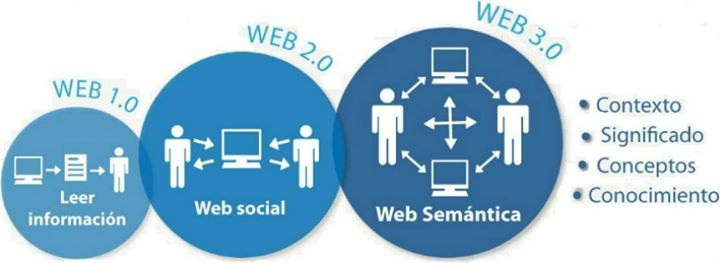
\includegraphics[width=0.7\linewidth]{imagenes/capitulo3/WEB}
	\caption{Evolución de la Web Semántica}
	\label{fig:web}
\end{figure}

% FUNCIONALIDAD WEB ACTUAL

% Apuntes clase Jose
% COURSERA: La Web Semántica: Herramientas para la publicación y extracción efectiva de información en la Web
Una de las principales causas del éxito de la Web se debe a la implantación como formato universal del lenguaje HTML (Figura \ref{html}). Gracias a este lenguaje, los ordenadores pueden analizar la estructura de las páginas Web, determinar cuál es la cabecera o indicar dónde hay un enlace a otra página. Sin embargo, no tienen una manera fiable de procesar la semántica de las páginas, lo que convierte a la Web actual en una Web Sintáctica cargada de documentos HTML diseñados sólo para ser leídos por humanos \cite{apuntes-clase-jose}.\\

La Web Sintáctica, la que usamos actualmente, hace alusión a la búsqueda de información sin interpretación del significado. Por ejemplo, si se escribe en Google la frase ``\textit{la buena lectura}'', el navegador buscará en que páginas aparecen esas tres palabras, es decir, dicha búsqueda se hace sin tener en cuenta el significado que pueda tener la frase. Por ejemplo, en la figura \ref{ejemplo} podemos apreciar como dicha búsqueda nos devuelve páginas en cuyo título aparecen al menos dos de las tres palabras de nuestra frase. Esto se debe a que el enfoque clásico de buscar en la Web se basa en similitudes y sinónimos generales de texto y palabras, además de en el uso de estadísticas, lo que dificulta limitar los resultados que un usuario desea. De esta manera, el usuario debe seguir un proceso iterativo para encontrar las palabras clave adecuadas para la obtención de los resultados esperados.

\begin{figure}[H]
	\centering
	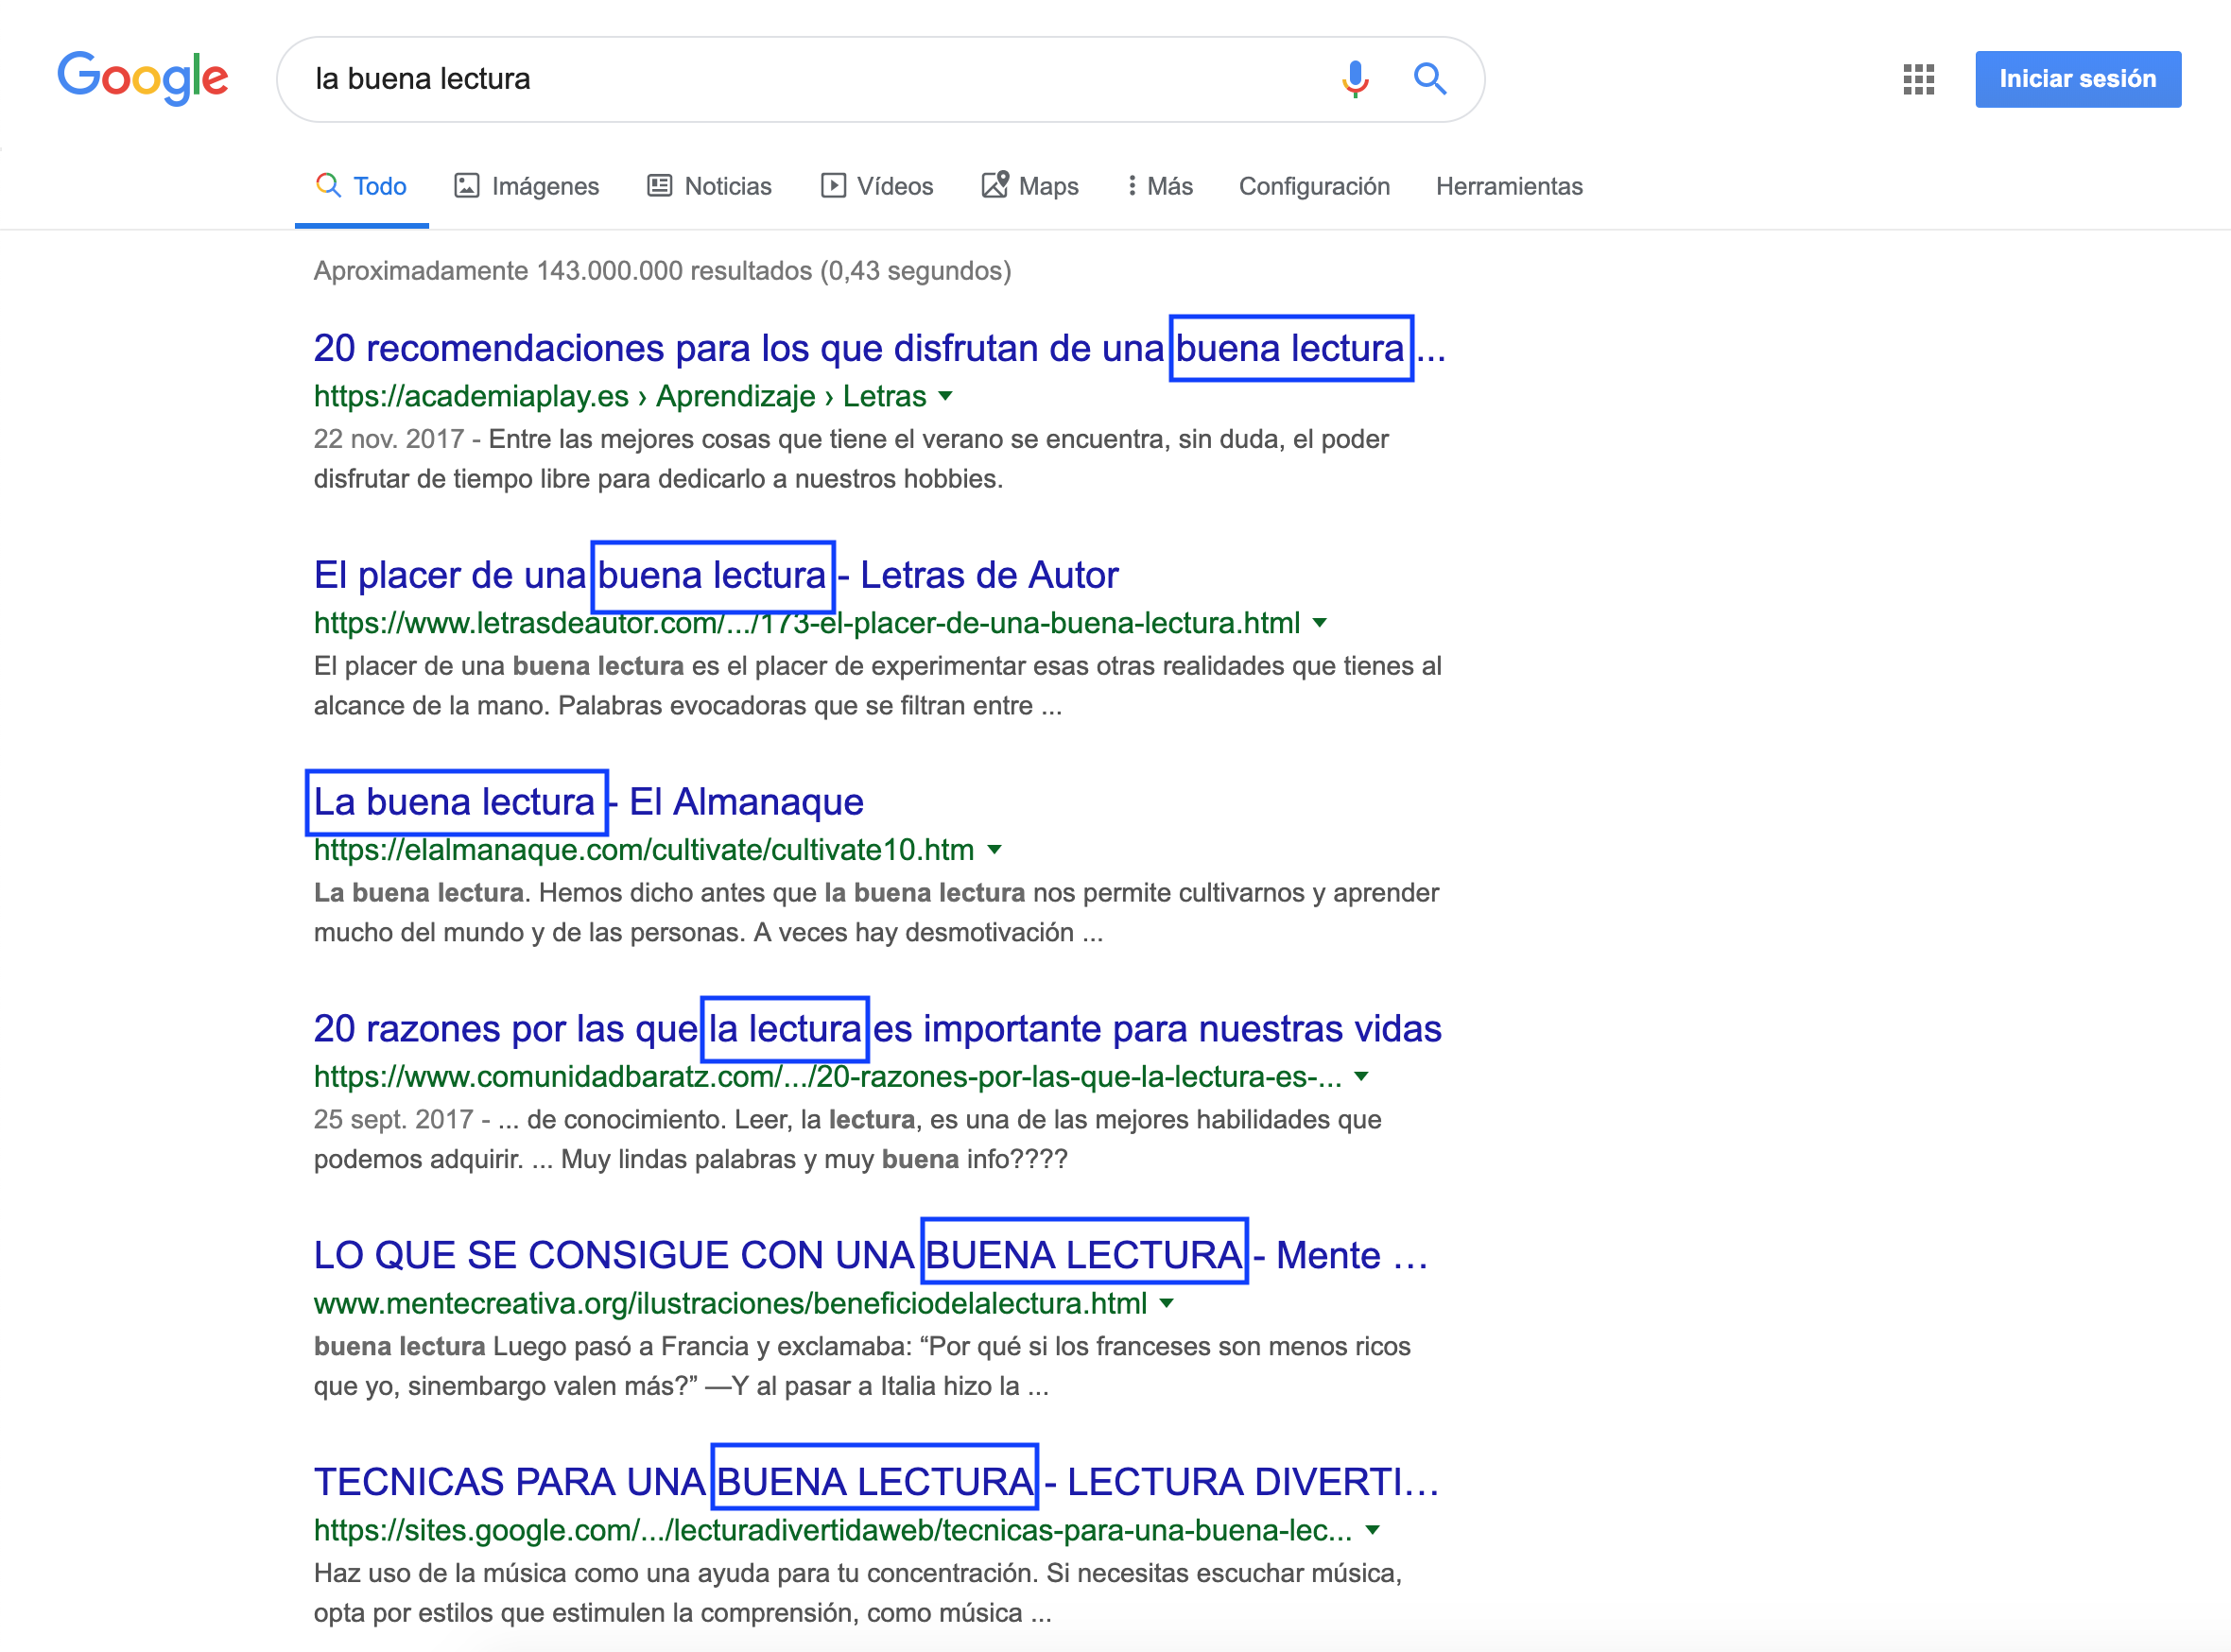
\includegraphics[height=9.5cm]{imagenes/capitulo3/ejemplo}
	\caption{Ejemplo de la búsqueda ``\textit{la buena lectura}'' en Google}
	\label{ejemplo}
\end{figure}

Otro ejemplo para la Web podría ser el mostrado en la figura \ref{fig:wikipedia}, en donde podemos ver una página Web (Wikipedia) con la descripción de la WWW \cite{coursera}. La mayoría de nosotros estamos familiarizados con Wikipedia, y cuando accedemos a ella no nos supone mucha dificultad distinguir su contenido textual, sus imágenes o sus enlaces en color azul para redirigirnos a otras páginas Web con otros contenidos totalmente distintos. Entonces \textit{¿cómo podría una aplicación consumir datos de dos Webs distintas?} o \textit{¿cómo sabría qué contenido leer dentro de cada página Web?} Ambas preguntas podrán ser contestadas una vez finalizado el presente trabajo.

\begin{figure}[H]
	\centering
	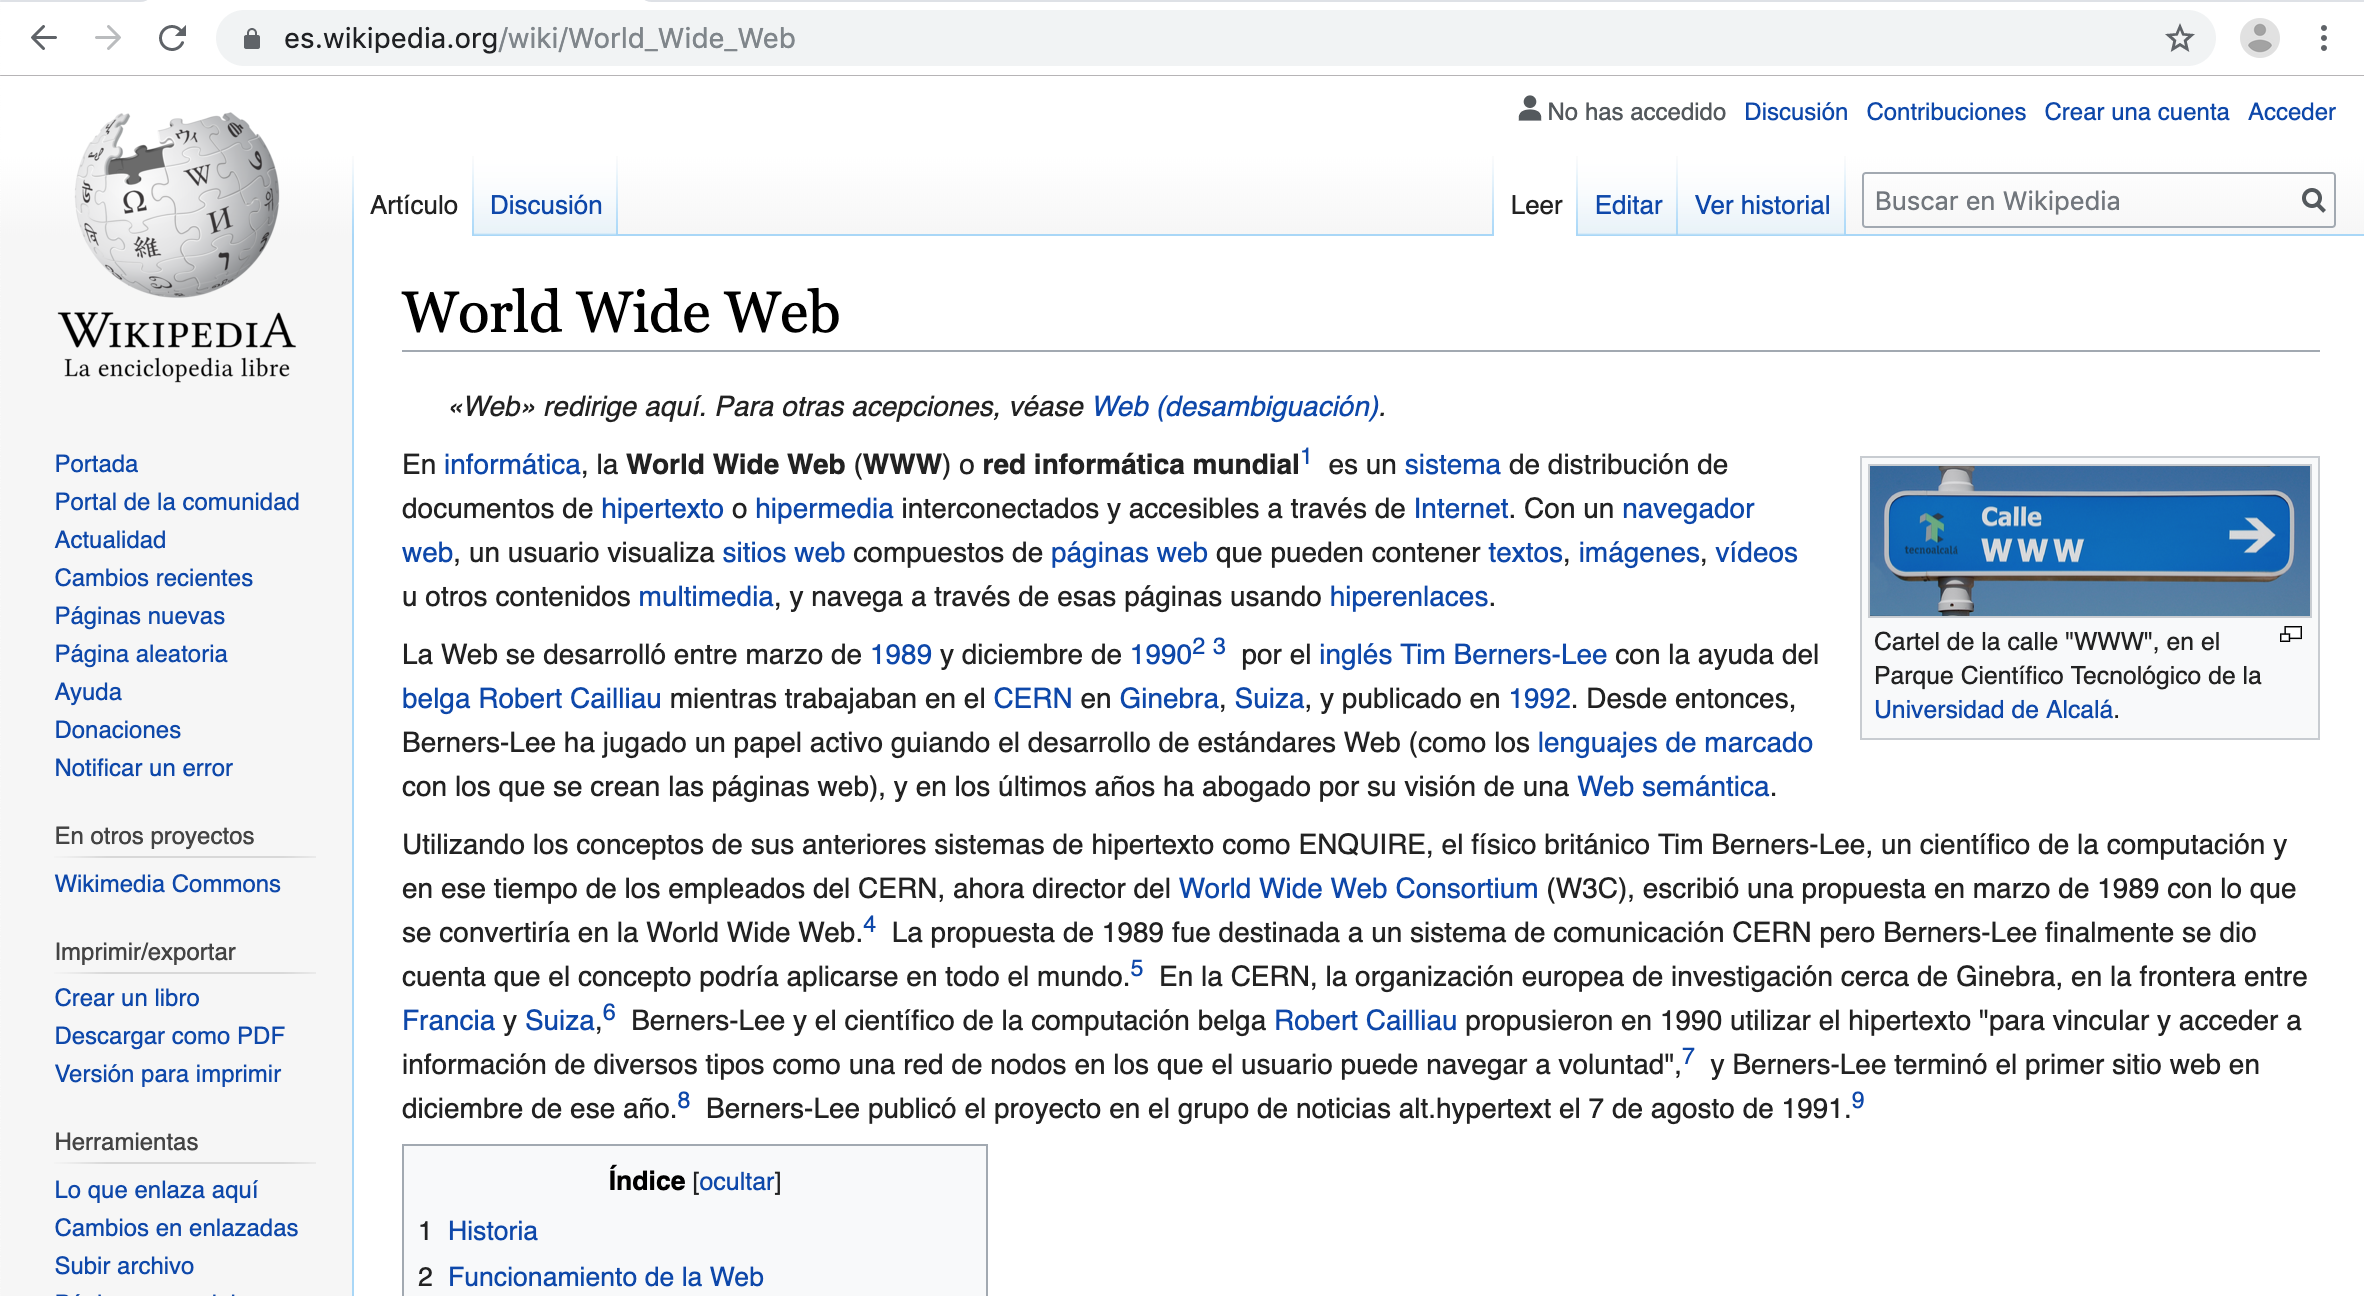
\includegraphics[height=6.95cm]{imagenes/capitulo3/wikipedia}
	\caption{Entrada en Wikipedia para la WWW}
	\label{fig:wikipedia}
\end{figure}


% EJEMPLO 1 DE WEB ACTUAL


% Leyendo el texto, el contenido. Pero, ¿cómo sabe qué contenido leer dentro de una página web? Mirando el código HTML de cada página. Podría ser pero es muy desordenado. Por dentro el código está muy desordenado siempre. Uno no sabe, una aplicación no sabría exactamente dónde está el nombre de una persona dentro del código html. Normalmente es muy difícil de saber.

% http://www.fgcsic.es/lychnos/es_es/articulos/construyendo_una_web_semantica
%Todos estamos bastante familiarizados con la Web y cómo operar con ella. Abrimos un navegador (por ejemplo, Chrome, Explorer, Firefox o Safari) e introducimos la dirección de la página que deseamos consultar o bien pedimos a un buscador (por ejemplo Google, Bing o Yahoo!) que nos determine las ubicaciones de documentos en la Web que contengan una combinación de palabras deseada y que nos las ordene por importancia.­


% http://www.bibliopos.es/Biblion-A2-Bibliografia-Documentacion/18ontologia-Web-Semantica.pdf
% https://www.w3c.es/Eventos/2009/Talleres/Murcia/Presentaciones/jesualdo.pdf

% [ejemplo arquitectura de como funciona la web actual]
% [mencionar algo de pubmed]

% ENTIENDO QUE ES LA WEB ACTUAL
% DESAFÍOS QUE PRESENTA LA WEB ACTUAL

% COURSERA: La Web Semántica: Herramientas para la publicación y extracción efectiva de información en la Web
Seguidamente, una vez entendida la Web actual, es necesario comprender los desafíos que presenta (tabla \ref{desafios}). Para ello debemos empezar diciendo que la Web actual es masiva (\textit{¿cuántos millones de páginas Web existen en la red?}), cambiante (\textit{¿cuántos tweets se generan en un segundo?}), heterogénea (\textit{¿cuántos millones de dispositivos independientes generan datos en un día?}) y está hecha para humanos \cite{coursera}.

\begin{table}[H]
	\centering
	\caption{Desafíos que presenta la Web actual \cite{coursera}}
	\label{desafios}
	\begin{tabular}{|>{\columncolor[HTML]{EFEFEF}}l |m{7.75cm}|}
		\hline
		\textbf{Heterogénea} & Múltiples organizaciones generan datos de forma independiente \\ \hline
		\textbf{Masiva} & La cantidad de información existente es enorme \\ \hline
		\textbf{Cambia muy rápido} &  Cada día son publicados y borrados enormes
		vólumenes de información\\ \hline
		\textbf{Hecha para humanos} &  En general, una persona puede interpretar la información de una página Web\\ \hline
	\end{tabular}
\end{table}



%\begin{figure}[H]
%	\centering
%	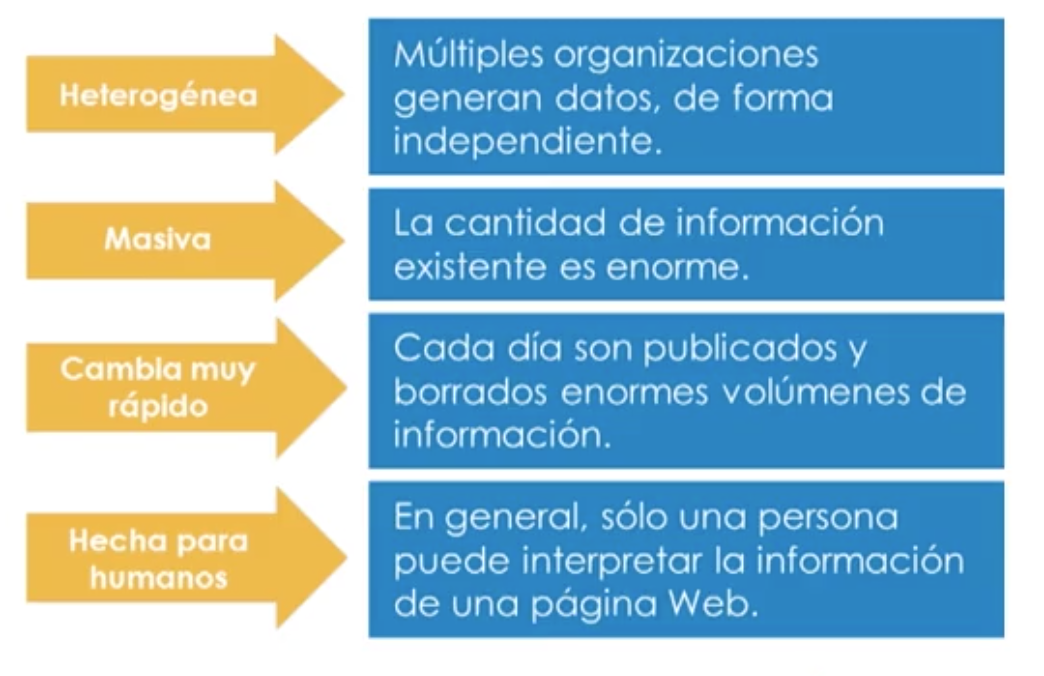
\includegraphics[height=6cm]{imagenes/capitulo3/1} % Características de la WEB
%	\caption{}
%	\label{desafios}
%\end{figure}



%\begin{enumerate}

% Heterogenea
% El primer desafío es la heterogeneidad. Como hemos visto, la Wikipedia tiene un formato, PubMed tiene otro formato, Facebook tiene otro formato de datos, nos presenta las cosas de forma distinta. Es decir la web es muy heterogénea.
%\item \textbf{Heterogénea}: ¿Cuántos millones de dispositivos independientes generan datos en un día? En la red existen muchas páginas web que son capaces de generar mucha cantidad de datos, y presentarlos de manera totalmente distinta a los usuarios. Por ejemplo, las redes sociales como 
%Tanto las páginas web como aplicaciones web generan muchos datos, los cuales y los presenta de manera totalmente distinta a los usuarios. No es lo mismo lo que se hace en todas las redes sociales, como por ejemplo Twitter o Facebook, ya que son totalmente distintas y no intercambian datos entre ellas.

% Masiva
% ¿Y cómo es la web actual? Primero la web actual es masiva. 
% Además la web es masiva. Hay muchísimos datos en PubMed, en Wikipedia, en Facebook. Hay una cantidad ingente de datos. Además cambia muy rápido. Por ejemplo, yo podría estar actualizando mi perfil de Facebook cada hora, cada dos horas. Hay gente que lo actualiza cada 15 minutos. Entonces todo esto cambia muy rápido y estoy dando un ejemplo muy chiquito, muy concreto. Además la web es masiva. Por ejemplo, la Wikipedia son casi 6 terabytes de datos. Y ¿qué es un terabyte de datos? En un terabyte de datos caben 678 millones de páginas de texto. 678 millones, eso, suponiendo que el Quijote tiene 1.000 páginas de texto, quiere decir que en un terabyte caben 678 mil Quijotes, Y en una Wikipedia, con 6 terabytes de datos, caben alrededor de 4 millones de Quijotes. Muchísimo.

%\item \textbf{Masiva}: ¿Cuántos millones de páginas web existen? Hoy en día, páginas como Wikipedia o Twitter generan muchísimos datos cambiantes. Por ejemplo, es posible estar actualizando mi perfil cada hora. 

% Cambia muy rápido
%  Además la web actual es cambiante  ¿Cuántas actualizaciones de perfil de Facebook se generan? Incontables,
% Esos son 27 Wikipedias por segundo. Se transfieren alrededor de Internet 27 Wikipedias cada segundo. Eso es muchísimo.
%\item \textbf{Cambia muy rápido}: ¿Cuántos tweets por segundo se generan? Actualmente se transfieren en Internet 160 terabytes de datos por segundo, lo que genera que cambie muy rápido. 

% Hecha para humanos
% La web actual además es distribuida, cualquier persona en el mundo puede acceder o generar contenido, no solo esto la web actual es un gran repositorio de información al cual todo el mundo puede acceder.
% Además la web está hecha para humanos. Como comentaba anteriormente Facebook lo consumen principalmente las personas. La Wikipedia la consumen normalmente las personas. Pero ¿qué pasa si yo quiero enlazar o combinar los datos de la Wikipedia y de Facebook o la Wikipedia y de PubMed? Eso actualmente, con el diseño de la web actual no es posible.
%\item \textbf{Hecha para humanos}: Si nos hemos fijado hasta el momento, los ejemplos que he puesto, la Wikipedia, Twitter o Facebook, están hechas para que sean consumidos por las personas. Las máquinas, el software no tiene tanto acceso a este contenido. Es difícil para un programa interpretar los datos que hay, por ejemplo, en el perfil de Facebook de una persona. o dentro de la Wikipedia. 

%\end{enumerate}

% ENTENDER LA WEB ACTUAL (RESUMEN DEL PARRAFO)
% INTRODUCIR AL FINAL LA WEB SEMÁNTICA (VER COMO HACERLO) Y ASÍ UNIRLO AL SIGUIENTE APARTADO

% https://disenowebakus.net/semantica-web.php
% COURSERA: La Web Semántica: Herramientas para la publicación y extracción efectiva de información en la Web
% LA ONTOLOGÍA Y LA WEB SEMÁNTICA: RECOMENDACIONES DEL W3C. 
% RAE
% Apuntes clase Jose

En consecuencia, podemos concluir que la Web se ha impuesto como el instrumento de uso cotidiano más potente y rápido para el intercambio y/o difusión de información en nuestra sociedad, accesible toda ella a través de Internet. No obstante, su capacidad para satisfacer necesidades específicas es limitada. Entonces, \textit{¿es realmente accesible esta información?} Hoy en día, existen numerosas herramientas como Google, Yahoo! o Bing que nos facilitan el acceso a esos datos \cite{semantica-web}. Sin embargo, estas herramientas tienen dificultades a la hora de entender la información que está contenida en ellas. Asimismo, la abrumadora obtención de resultados, tanto relevantes como irrelevantes a partir de una búsqueda, denota una importante falta de precisión en la Web \cite{coursera}. Este inconveniente se debe principalmente a que la Web actual carece de capacidad para expresar significados. En particular, estas herramientas miran las páginas Web como si fueran un conjunto de palabras, limitándose a recoger cadenas de caracteres indexadas en grandes bases de datos o a buscar palabras clave, y presentarlas en la pantalla del ordenador para su posterior visualización (Figura \ref{ejemplo}) \cite{web-semantica-w3c}. Por lo cual, estas herramientas no son capaces de entender los elementos que forman parte de ella (lugares geográficos, actores, películas) y las relaciones existentes entre estos elementos, lo que dificulta que el ordenador no sepa realmente lo que significa la información, puesto que la mayoría de los contenidos de la Web actual están diseñados para ser leídos por humanos \cite{apuntes-clase-jose}. \\

% tesis
%En la actualidad, la Web esta compuesta por varios documentos distribuidos en diferentes lugares del planeta, durante muchos años ha sido una poderosa herramienta para publicar, buscar y compartir información  convirtiéndose en una gran base de datos, siendo imposible explotar adecuadamente esa información. 
%\begin{figure}[H]
%	\centering
%	\includegraphics[height=5.6cm]{imageness/capitulo3/bing} 
%	\caption{Página inicial del buscador Bing}
%	\label{bing}
%\end{figure}

%\begin{figure}[H]
%	\centering
%	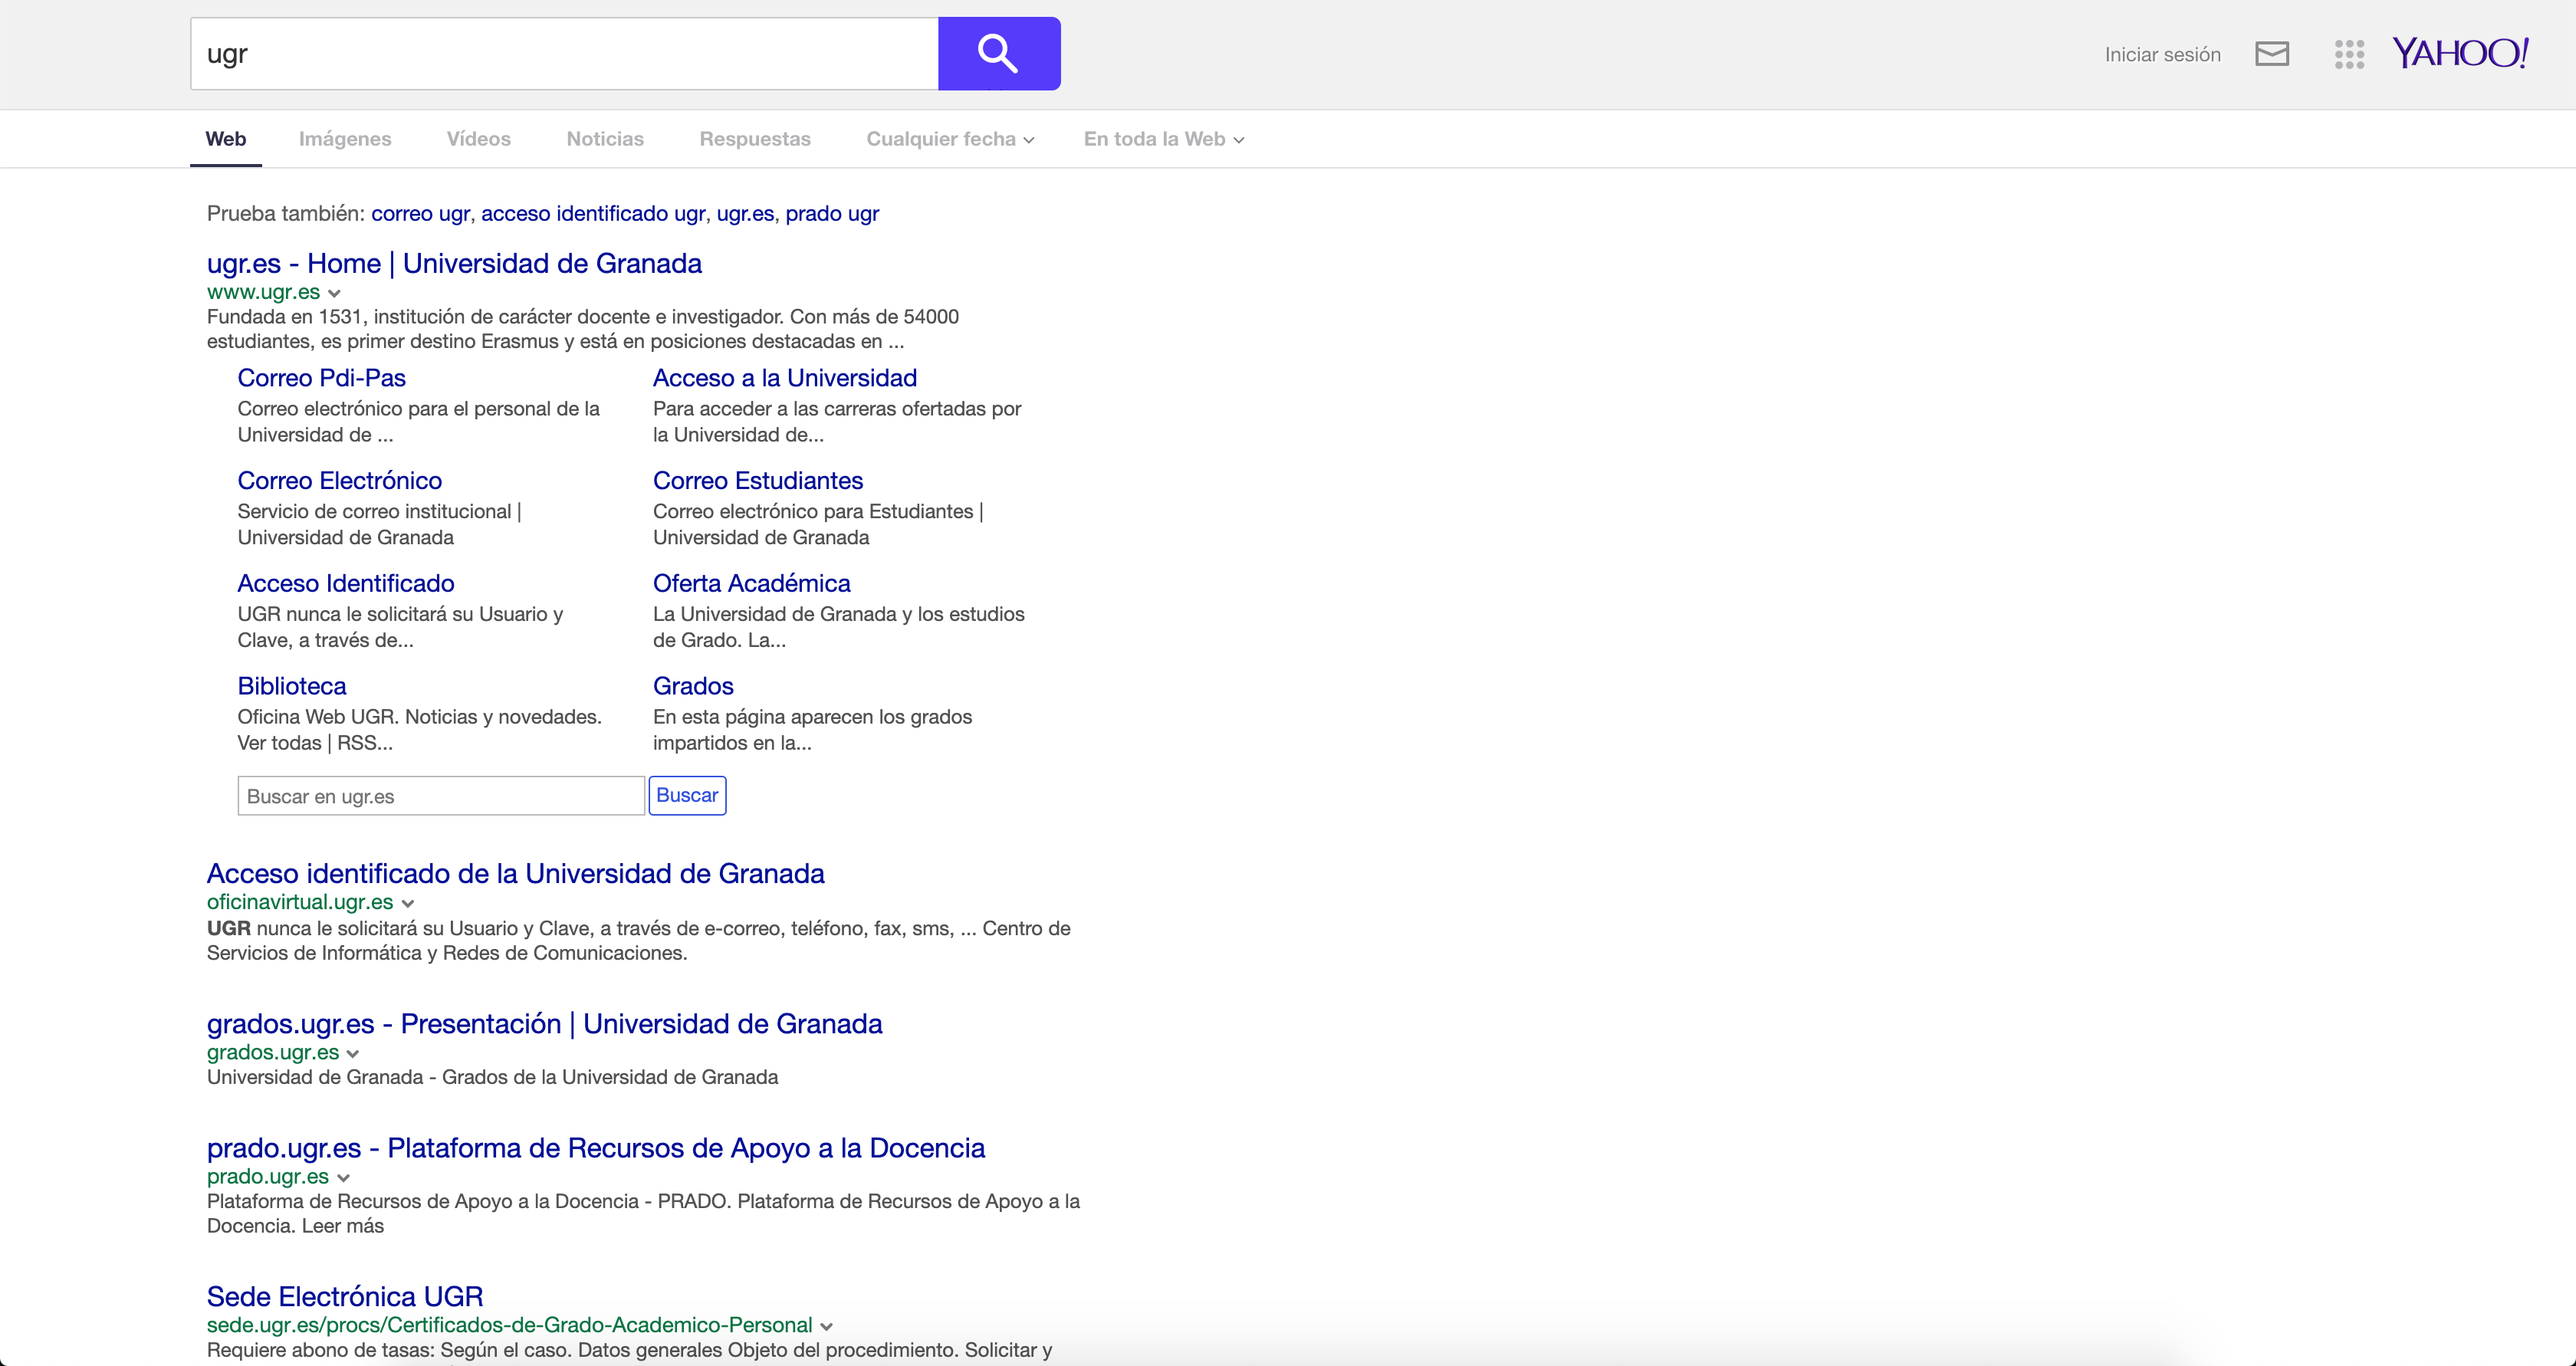
\includegraphics[height=6.7cm]{imagenes/capitulo3/yahoo-busqueda} % https://www.google.com/search/howsearchworks/
%	\caption{Búsqueda de ``ugr'' en Yahoo}
%	\label{yahoo-busqueda}
%\end{figure}

% Apuntes clase Jose
% COURSERA: La Web Semántica: Herramientas para la publicación y extracción efectiva de información en la Web
Por esta razón surge la Web Semántica, para proporcionar estructura al contenido semántico de las páginas Web, con la finalidad de que los contenidos puedan ser consumidos por máquinas de manera más eficiente. En el siguiente subapartado entramos en detalle en el concepto de Web Semántica.

\subsection{Concepto de Web Semántica} 

Para comprender que es la Web Semántica (\url{ www.semanticweb.org}), es necesario establecer los principios básicos sobre los que se asienta (figura \ref{fig:principio}). En el subapartado anterior se estableció el contexto en el que nace, a continuación se procede a explicar su definición. 

\begin{figure}[H]
	\centering
	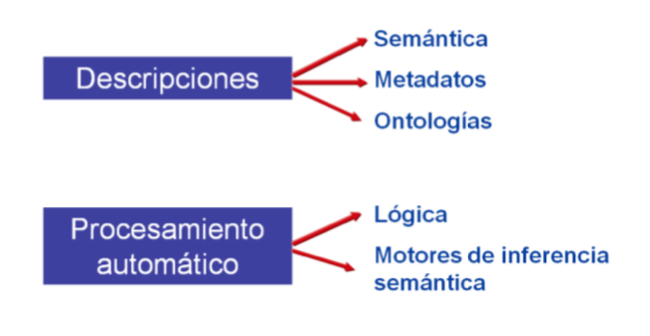
\includegraphics[width=0.57\linewidth]{imagenes/capitulo3/principio}
	\caption{Principios básicos de la Web Semántica \cite{aplicacion}}
	\label{fig:principio}
\end{figure}

La \textbf{Web Semántica} es una corriente promovida también por Tim Berners-Lee, cuyo fin es lograr que las máquinas puedan entender y, por tanto, utilizar lo que la Web contiene. De ahí que se haya tomado el término \textit{semántica}, que desde el punto de vista lingüístico ``\textit{es la disciplina que estudia el significado de los términos}'' \cite{cwb}. Esta idea surge a raíz de un artículo publicado por la revista \textit{Scientific American} en mayo de 2001, en donde Tim Berners-Lee propone una nueva forma de organizar el contenido en la Red para superar el problema de la heterogeneidad semántica y proporcionar a las computadoras contenidos Web significativos \cite{web-semantica-w3c, libro-gis}.\\


% EMPEZAMOS A DEFINIR - PRIMERA DEFINICIÓN LA OFICIAL (VER OTRAS DE LA LITERATURA)


% LA ONTOLOGÍA Y LA WEB SEMÁNTICA: RECOMENDACIONES DEL W3C. 
% http://www.fgcsic.es/lychnos/es_es/articulos/construyendo_una_web_semantica


% COURSERA: La Web Semántica: Herramientas para la publicación y extracción efectiva de información en la Web
% https://www.researchgate.net/publication/216537707_La_Web_semantica_y_las_tecnologias_del_lenguaje_humano
% https://disenowebakus.net/semantica-web.php
% LA ONTOLOGÍA Y LA WEB SEMÁNTICA: RECOMENDACIONES DEL W3C. 
% de descentralización, máxima facilidad de acceso y/o apertura al crecimiento
En palabras de Tim Berners-Lee \cite{researchgate}: ``\textit{La Web Semántica es una extensión de la actual Web en la que a la información disponible se le otorga un significado bien definido que permita a los ordenadores y a las personas trabajar en cooperación. Está basada en la idea de proporcionar en la Web datos definidos y enlazados, permitiendo que aplicaciones heterogéneas localicen, integren, razonen y reutilicen la información presente en la Web}''. Considerando la definición aquí aportada, la Web Semántica se manifiesta como una evolución de la actual Web, no una sustitución ya que mantiene sus características principales (descentralización, facilidad de acceso), en donde los ordenadores son capaces de interpretar los documentos; sin hacer uso de Inteligencia Artificial ya que la semántica se encuentra en las páginas \cite{semantica-web}. \\

% OTRA DEFINICIÓN - W3C

% COURSERA: La Web Semántica: Herramientas para la publicación y extracción efectiva de información en la Web
% https://www.researchgate.net/publication/216537707_La_Web_semantica_y_las_tecnologias_del_lenguaje_humano
% https://disenowebakus.net/semantica-web.php
% LA ONTOLOGÍA Y LA WEB SEMÁNTICA: RECOMENDACIONES DEL W3C. 
% https://disenowebakus.net/semantica-web.php
Pero, \textit{¿cómo se traduce lo que acabamos de definir a la práctica?} En la práctica, la Web Semántica es un conjunto de recomendaciones\footnote{Una recomendación es una descripción formal de una tecnología que debe ser utilizada por todos.} desarrolladas por el \textbf{World Wide Web Consortium}\textbf{ (W3C) }que es el organismo encargado de velar por la normalización en Internet y dictar los distintos estándares para la Web. El objetivo principal de este organismo reside en ``\textit{guiar a la Web hacia su máximo potencial mediante el desarrollo de protocolos y pautas comunes que promuevan su evolución y garanticen su interactividad}’’ \cite{coursera, web-semantica-w3c}. Dentro de la página oficial del W3C (\url{https://www.w3.org}), podemos encontrar otra definición para la Web Semántica: ``\textit{La Web Semántica es la representación de datos en la Web. Es un esfuerzo colaborativo liderado por W3C con la participación de un gran número de investigadores y socios industriales. Se basa en el uso de RDF, que integra una gran variedad de aplicaciones mediante el uso de XML, para la sintaxis y el uso de URLs para su identificación}'' \cite{semantica-web}. Considerando la definición expuesta, los términos mencionados aquí se escapan de los conocimientos aprendidos hasta ahora, en donde las tecnologías nombradas serán tratadas en sucesivos apartados, ya que la W3C recomienda el uso de RDF (\textit{Resource Description Framework}) y OWL (\textit{Ontology Web Language}) para la construcción de la Web Semántica.\\

% tesis
% INTRODUCCIÓN A LA WEB SEMÁNTICA: REALIDADES Y PERSPECTIVAS.
% COURSERA: La Web Semántica: Herramientas para la publicación y extracción efectiva de información en la Web
De igual manera, nos encontramos a lo largo de la literatura más definiciones de Web Semántica, si bien todas guardan un nexo en común y es el de dotar de mayor significado a la Web actual a través de lenguajes universales que resuelvan los problemas ocasionados por una Web carente de semántica en la que a veces el acceso a la información se convierte en una tarea difícil \cite{introduccion}. Para ello, se desarrollan y usan lenguajes que facilitan la introducción en la Web de contenido legible por las máquinas \cite{tesis}. Entonces, \textit{¿cuáles son los requisitos esenciales para que una Web de datos pueda ser accedida y entendida tanto por ordenadores como por personas?} \cite{coursera}:

\begin{enumerate}
	\item Se nescesita disponer de un l\textbf{enguaje que permita especificar los recursos de la Web y las relaciones que existen entre ellos}. Con esto, lo que se pretende es desarollar una Web más cohesionada en donde sea más fácil localizar, compartir e integrar información para sacar un mayor partido a los recursos disposibles. Para conseguir este objetivo es necesario que un sistema automático sea capaz de sacar sus propias conclusiones respecto a las búsquedas realizadas.
	
	\item Se necesita poder consultar esos datos mediante aplicaciones computacionales. Para ello es necesario disponer de un \textbf{lenguaje para describir consultas procesables por un computador} para su entendimiento y ser capaz de sacar conclusiones a partir de los datos de manera automática. Con esto se pretende explorar la Web de forma más automática y obtener resultados más enfocados.
\end{enumerate}

\begin{figure}[H]
	\centering
	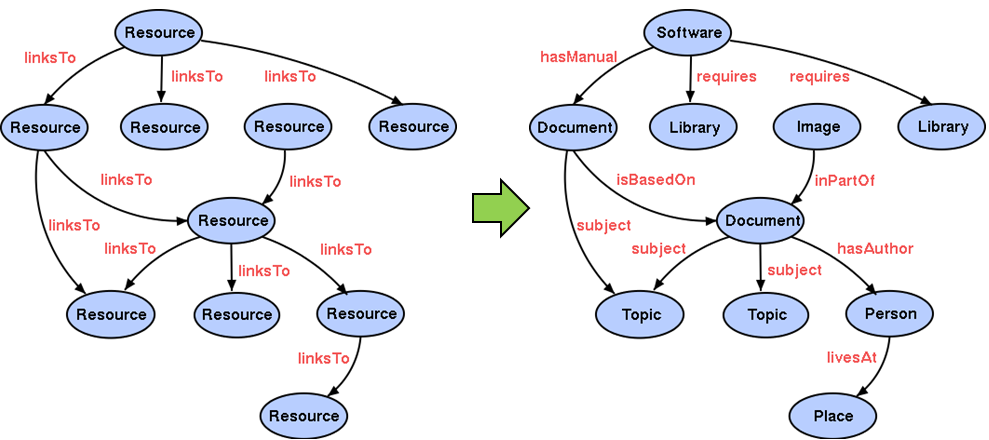
\includegraphics[height=5.60cm]{imagenes/capitulo3/web-actual-web-semantica.png}
	\caption{Web Sintáctica vs. Web Semántica}
	\label{wa-ws}
\end{figure}

% https://www.researchgate.net/publication/216537707_La_Web_semantica_y_las_tecnologias_del_lenguaje_humano
A partir de los conceptos explicados hasta ahora, la implantación de la Web semántica frente a la actual Web supone un cambio de paradigma, ya que tiene que pasarse de una Web basada y creada en lenguaje natural a una Web estructurada y organizada, en donde los contenidos etiquetados semánticamente serán el elemento principal \cite{researchgate}. En la figura \ref{wa-ws} podemos ver la diferencia que hay entre ambos tipos de Web. Se observa como el esquema de la izquierda de la actual Web está basado en los enlaces con los que accedemos a otras páginas, mientras que en la Web Semántica (esquema de la derecha) disponemos de información relevante.

\begin{figure}[H]
	\centering
	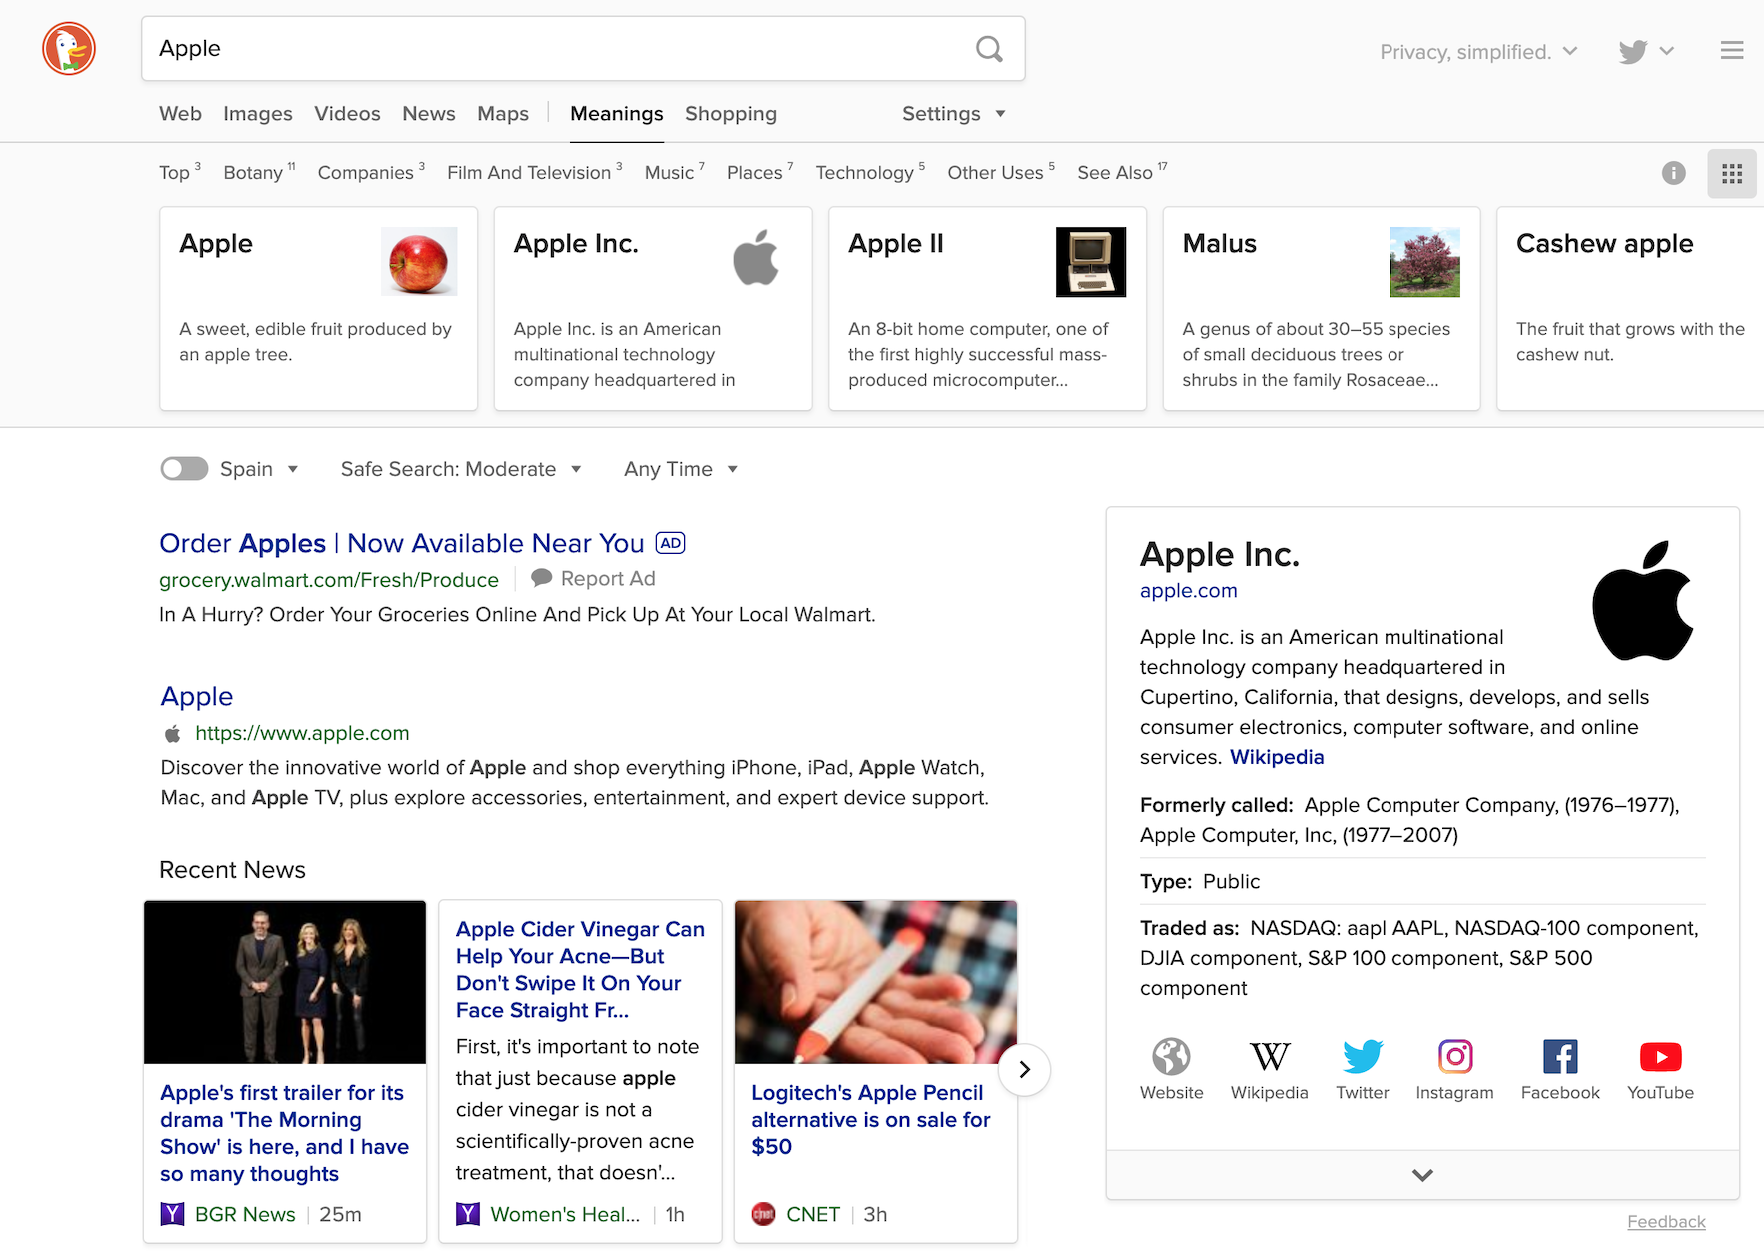
\includegraphics[height=9.cm]{imagenes/capitulo3/duck21}
	\caption{Búsqueda semántica de ``Apple'' en DuckDuckGo}
	\label{busqueda-semantica}
\end{figure}



% https://www.makeuseof.com/tag/top-7-semantic-search-engines-alternative-google-search/
% http://swoogle.umbc.edu/2006/ no funciona 
Por otro lado, para comprender los conceptos hasta aquí tratados, vamos a ver un ejemplo de buscador semántico. En Internet existen muchos buscadores de este tipo, de entre todas las posibilidades revisadas \cite{buscadores-semanticos} nos hemos quedado con dos: \textit{Swoogle} (\url{http://swoogle.umbc.edu/2006/}) y \textit{DuckDuckGo} (\url{https://duckduckgo.com/?t=h_}), pero debido a que el primero no ha funcionado, hemos hecho una pequeña demostración con el segundo. \textbf{DuckDuckGo} es un motor de búsqueda semántico rico en funciones, tiene innumerables razones para dejar atrás a Google. Respecto a las búsquedas, podemos encontrar una búsqueda clásica, búsqueda de información y/o compras, entre otros. Si se busca un término que tiene más de un significado, nos da la oportunidad de elegir lo que estamos buscando originalmente, con sus distintos resultados o significados. Por ejemplo, la búsqueda del término \textit{Apple}, en un navegador con idioma inglés, ofrece una larga lista de posibles significados, entre los que podemos destacar la fruta, la empresa tecnológica y muchos otros. Además, los clasifica en categorías, como se puede observar en la figura \ref{busqueda-semantica}. Sin embargo, la búsqueda para el término \textit{Apple} en un buscador sintáctico como puede ser Google, nos ofrece de primeras sólo la empresa tecnológica, ya que debido a estadísticas se obtiene que esa es la simlitud con mayor porcentaje para mostrar de primeras (figura \ref{busqueda-sintactica}).

\begin{figure}[H]
	\centering
	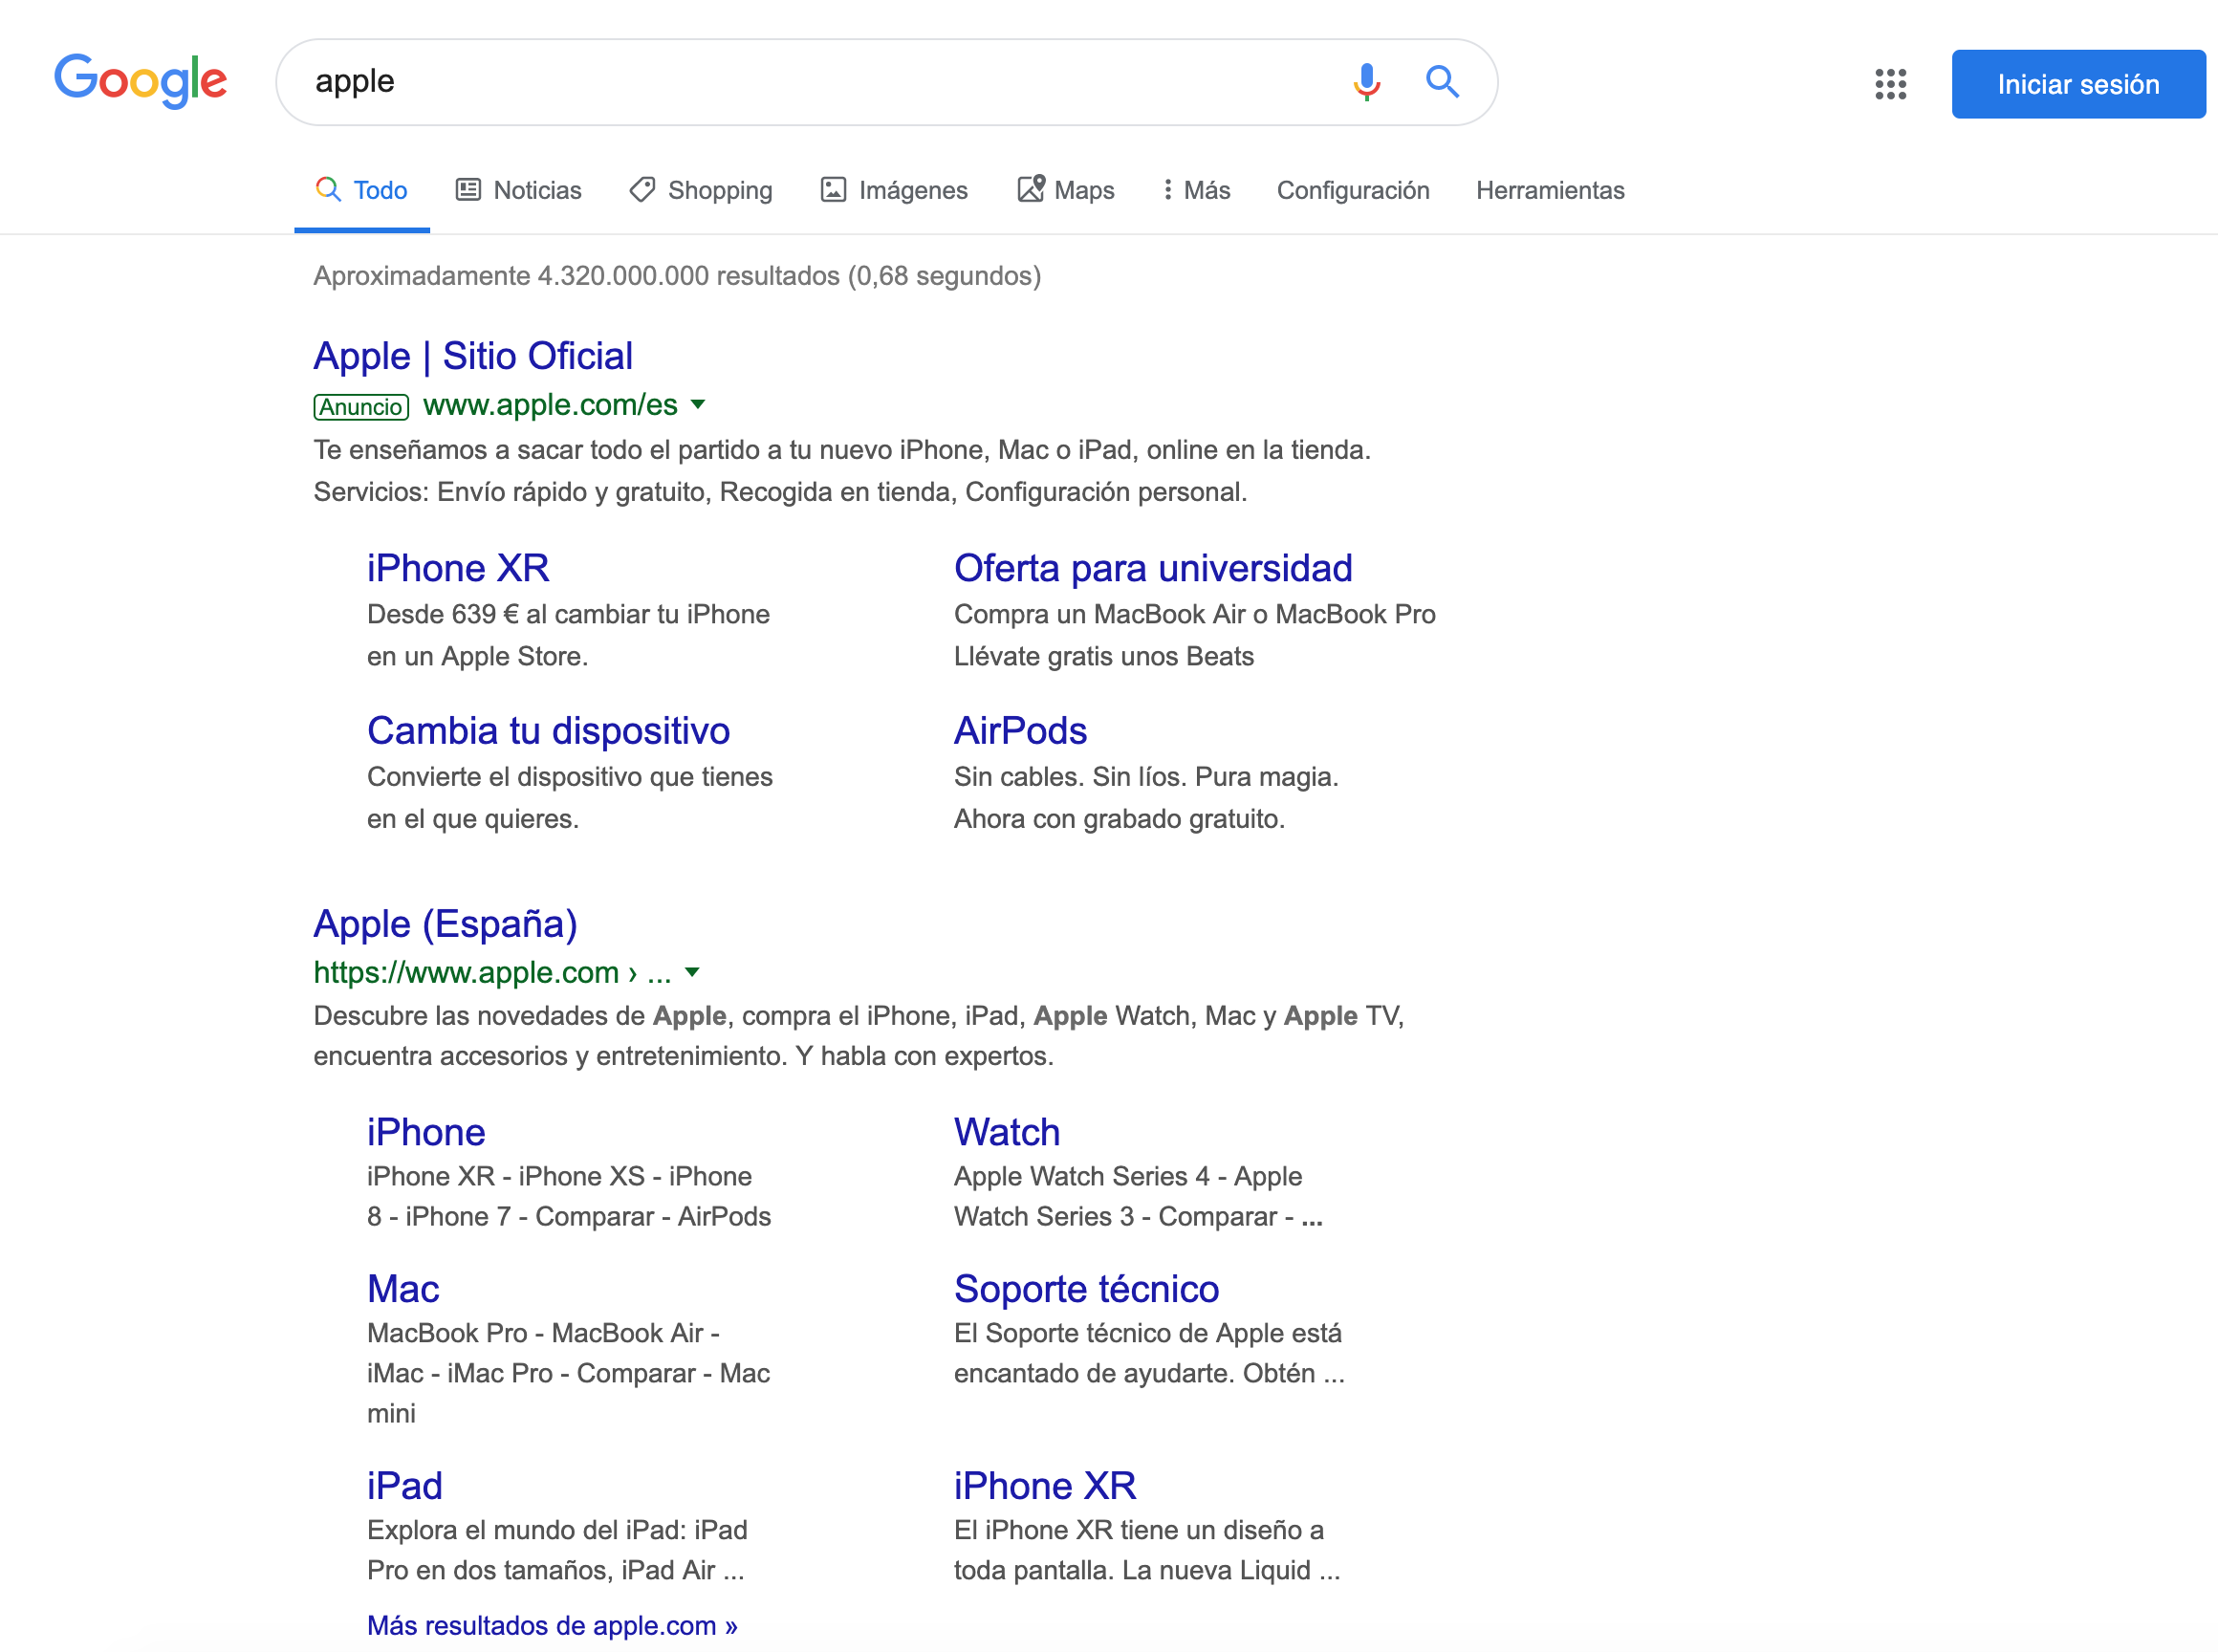
\includegraphics[height=9.4cm]{imagenes/capitulo3/apple}
	\caption{Búsqueda clásica de ``Apple'' en Google}
	\label{busqueda-sintactica}
\end{figure}

%\begin{figure}[H]
%	\centering
%	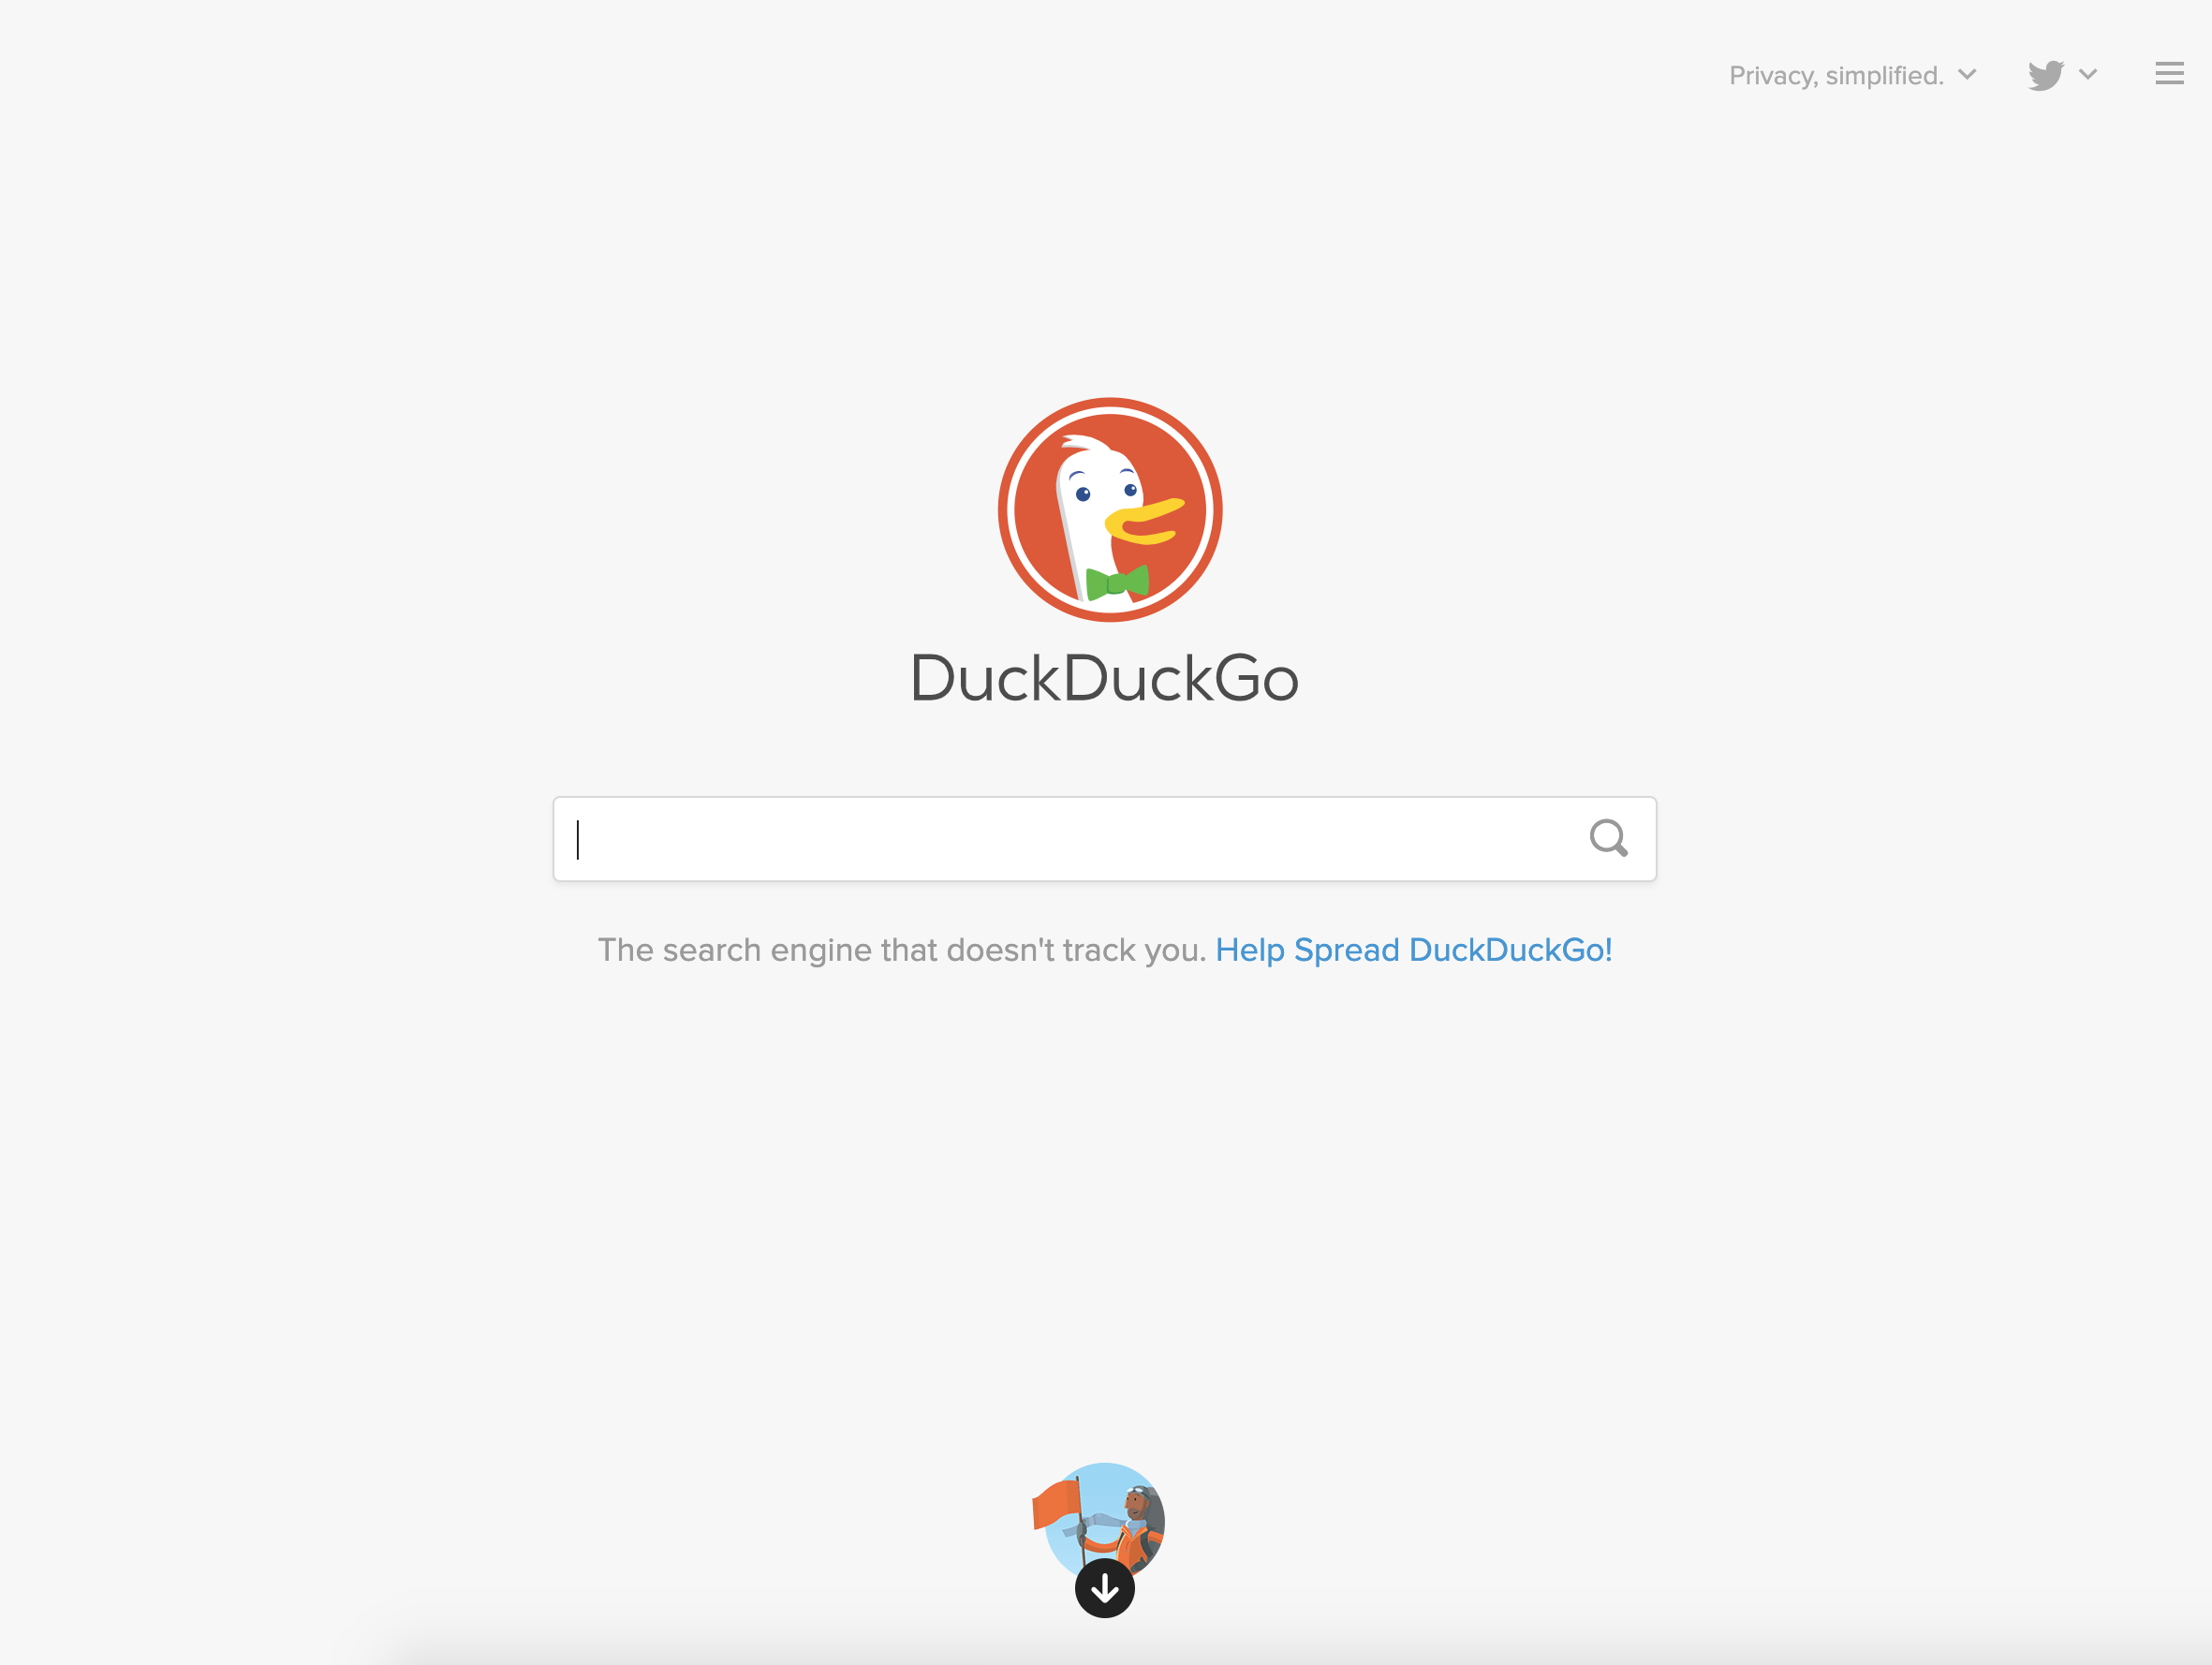
\includegraphics[height=8.5cm]{imagenes/capitulo3/duck1}
%	\caption{DuckDuckGo}
%	\label{DuckDuckGo}
%\end{figure}

Por tanto, después de haber analizado este ejemplo podemos concluir que la mayoría de los contenidos de la Web de hoy en día están diseñados para que los humanos los lean, no para que los programas de software procesen la semántica de manera significativa. Es por eso que nace la Web Semántica, para llevar estructuras a los contenidos significativos de las páginas Web y permitir que los programas de software procesen y comprendan los datos en las páginas. En donde, dichas tecnologías tratan de aportar información extra a los recursos Web, proporcionando contenidos con significado que permitan mejorar la interoperabilidad entre los Sistemas Informáticos \cite{aplicacion}. A través de la Web Semántica, los programas de software pueden usar colecciones estructuradas de información y conjuntos de reglas de inferencia para realizar razonamientos automatizados \cite{libro-gis}. \\

Con esto hemos terminado de definir el concepto de Web Semántica, a continuación se explican las capas que componen su arquitectura, tecnologías usadas en la prueba de concepto que se verá en el siguiente capítulo.


\section{Arquitectura de la Web Semántica}

% ARQUITECTURA 
% Capas de la Web Semántica

% https://www.researchgate.net/publication/216537707_La_Web_semantica_y_las_tecnologias_del_lenguaje_humano
\textit{¿Cuáles son los estándares para la Web Semántica?} En la figura \ref{fig:arquitectura1} se muestra la arquitectura de la Web Semántica tal y como la definió Berners-Lee. Se trata de una estructura de capas, donde cada nivel resulta un requisito previo para el siguiente \cite{researchgate}:

\begin{figure}[H]
	\centering
	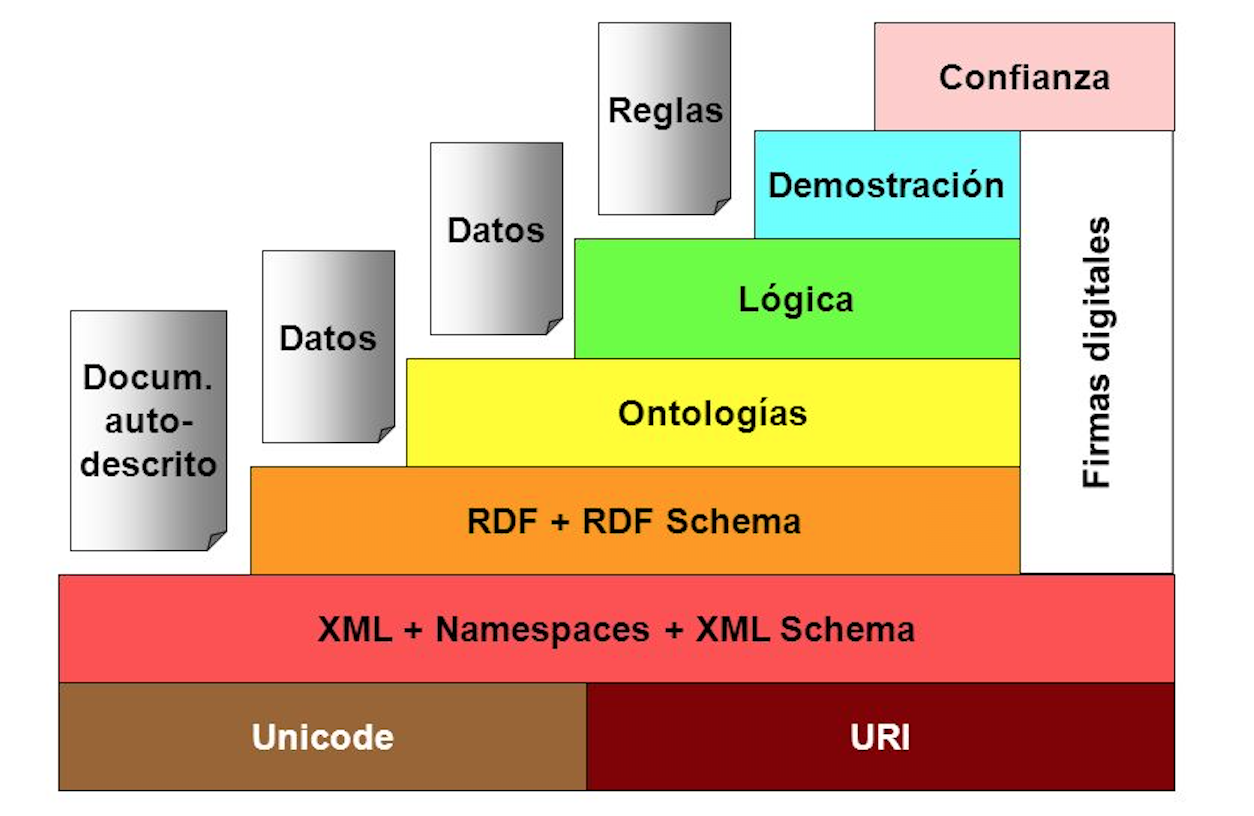
\includegraphics[width=0.7\linewidth]{imagenes/capitulo3/arquitectura1} 
	\caption{Modelo multicapa de la Web Semántica}
	\label{fig:arquitectura1}
\end{figure}

\begin{figure}[H]
	\centering
	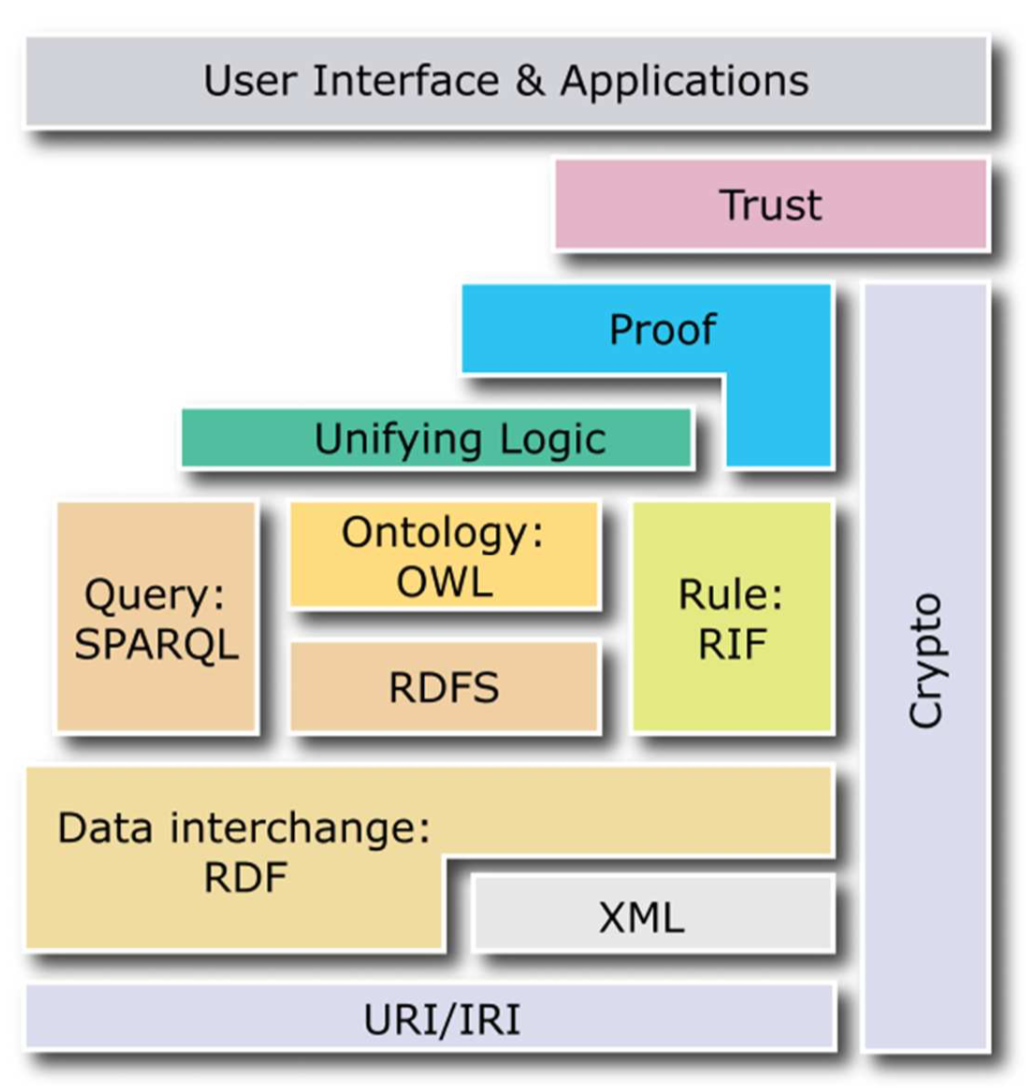
\includegraphics[width=0.55\linewidth]{imagenes/capitulo3/arquitectura2}
	\caption{Estructura de la Web Semántica}
	\label{fig:arquitectura2}
\end{figure}

% https://www.researchgate.net/publication/216537707_La_Web_semantica_y_las_tecnologias_del_lenguaje_humano
\begin{enumerate}
	\item \textbf{Unicode, URI, XML y RDF}: los tres primeros niveles hacen referencia a la base y los estándares en los que se sustenta su desarrollo, ya que permiten convertir la Web en una infraestructura global para compartir y reutilizar datos y documentos entre diferentes usuarios.
	
	\item \textbf{Ontologías}: capa donde reside el contenido semántico del sistema. 
	
	\item \textbf{Lógica}: en esta capa a partir de la estructura semántica generada con las ontologías y los metadatos, se realizan las inferencias lógicas; sin embargo, actúan como freno para la Web Semántica ya que comportan una infraestructura que actualmente es difícil de realizar a gran escala. 
	
	\item \textbf{Seguridad y Confianza}: los agentes deben ser escépticos de la información obtenida, y contrastar minuciosamente las distintas fuentes; podrán utilizar la firma digital para verificar que la fuente es confiable. 
	%las dos últimas capas más rápidas en implantarse, ya que la confianza y la seguridad son elementos clave de cualquier arquitectura, y se podrá usar la firma digital para verificar la fuente.
\end{enumerate}



La figura \ref{fig:arquitectura1} no es la única forma de representación de las capas de la arquitectura para la Web Semántica, sino que a lo largo de los años han surgido modelos similares. En el presente trabajo nos vamos a centrar en otro esquema (figura \ref{fig:arquitectura2}), el cual ha sido explicado en los cursos a los que he asistido durante este año. Así que a partir del esquema de la figura \ref{fig:arquitectura2}, vamos a describir las tecnologías o capas de carácter importante que se utilizan durante el desarrollo del presente trabajo: URI/IRI, XML, RDF, RDF Schema, Ontología (OWL) y SPARQL (GeoSPARQL).

% En este curso nos vamos a centrar en cuatro de estos componentes de esta pirámide que están marcados con colores. En primer lugar vamos a ver RDF, que es el lenguaje básico para especificar recursos de la web y sus relaciones, RDFS que nos permite decir un poco más vamos a hablar de este vocabulario, SPARQL que es este lenguaje de consulta que nos permite extraer información desde la web y finalmente OWL o este lenguaje que nos permite identificar ontologías.

\subsection{URI/IRI}

URI/IRI son los identificadores de la Web (figura \ref{fig:250px-irivenndiagramm}). Es el primer elemento necesario para el acceso a los recursos de la Web, los cuales pueden ser identificados unívocamente en cualquier idioma, a través del uso de Unicode e identificadores URI \cite{aplicacion}. El \textbf{URI} (\textit{\textbf{Uniform Resource Identifier}}) es una secuencia compacta de caracteres que identifican un recurso abstracto o físico que no tiene porqué existir en la Web. En la tabla \ref{uris} se observan algunos ejemplos de URIs \cite{uri}.

\begin{figure}[H]
	\centering
	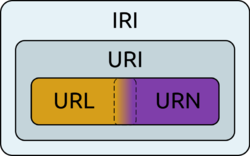
\includegraphics[width=0.4\linewidth]{imagenes/capitulo3/URI}
	\caption{Conjunto que englobas las IRI}
	\label{fig:250px-irivenndiagramm}
\end{figure}


\begin{table}[H]
	\caption{Ejemplos de URIs}
	\label{uris}
	\centering
	\begin{tabular}{|m{5.6cm}|m{5.6cm}|}
		\rowcolor[HTML]{EFEFEF} 
		\hline
		Ejemplo & Descripción \\ \hline
		\url{ftp://ftp.is.co.za/rfc/rfc1808.txt} & Esquema FTP para servicios de protocolo de transferencia de archivos\\ \hline
		%\url{http://www.math.uio.no/faq/compression-faq/part1.html} & esquema http para servicios de protocolo de transferencia de hipertexto\\ \hline
		\url{mailto:mduerst@ifi.unizh.ch} & Esquema MAILTO para direcciones de correo electrónico \\ \hline
		\url{telnet://melvyl.ucop.edu/} & Esquema TELNET para servicios interactivos a través del protocolo TELNET\\ \hline
	\end{tabular}
\end{table}

El \textbf{IRI} (\textit{\textbf{International Resource Identifier}}) se puede utilizar para encontrar diferentes tipos de recursos, como documentos, personas, objetos físicos y conceptos abstractos. Las URL que usamos como direcciones Web son una forma de IRI que sí existen en la Web. Además el IRI nace como como complemento del URI, debido a que los IRI son identificadores globales, los usuarios pueden reutilizarlos para identificar lo mismo \cite{libro-gis}.


%Son los identificadores de la Web, la URi no tiene porqué existir en la Web www.ugr.es/jsamos es existe es una URL, la URI no tiebe porque 

%Lo más genrico con los URI

% https://www.ietf.org/rfc/rfc3986.txt
% https://www.ietf.org/rfc/rfc3986.txt
%Un identificador uniforme de recursos (URI) es una secuencia compacta de caracteres que identifican un recurso abstracto o físico. Esta
%La especificación define la sintaxis genérica de URI y un proceso para resolviendo referencias de URI que podrían estar en forma relativa, junto con directrices y consideraciones de seguridad para el uso de URI en el Internet. La sintaxis de URI define una gramática que es un superconjunto de todos URI válidos, lo que permite una implementación para analizar los componentes comunes de una referencia URI sin conocer los requisitos específicos del esquema de cada posible identificador. Esta especificación no define un gramática generativa para URIs; esa tarea la realiza el individuo especificaciones de cada esquema URI.


% https://www.ietf.org/rfc/rfc3986.txt
%Este documento define un nuevo elemento de protocolo, el Internacionalizado Identificador de recursos (IRI), como complemento del recurso uniforme Identificador (URI). Un IRI es una secuencia de caracteres de Juego de caracteres universal (Unicode / ISO 10646). Un mapeo de IRIs a Se definen URI, lo que significa que se pueden usar IRI en lugar de URI, en su caso, para identificar recursos.

%Se eligió el enfoque de definir un nuevo elemento de protocolo en lugar de extender o cambiar la definición de URI. Esto se hizo en orden para permitir una distinción clara y evitar incompatibilidades con software existente Se proporcionan pautas para el uso y despliegue de IRI en varios protocolos, formatos y software componentes que actualmente tratan con URI.

% https://www.ietf.org/rfc/rfc3986.txt
%Los IRI están destinados a reemplazar los URI en la identificación de recursos para
%protocolos, formatos y componentes de software que usan un UCS
%repertorio de personajes. Es posible que estos protocolos y componentes nunca necesiten
%para usar los URI directamente, especialmente cuando se usa el identificador de recursos
%simplemente con fines de identificación. Sin embargo, cuando el recurso
%identificador se utiliza para la recuperación de recursos, en muchos casos
%necesario para determinar el URI asociado, porque actualmente la mayoría
%Los mecanismos de recuperación solo se definen para los URI. En este caso, IRI
%puede servir como elementos de presentación para elementos de protocolo URI. Un
%ejemplo sería una barra de direcciones en un agente de usuario web. (Adicional
%La justificación se da en la sección 3.1.)


%A URI can be further classified as a locator, a name, or both.  The
%term "Uniform Resource Locator" (URL) refers to the subset of URIs
%that, in addition to identifying a resource, provide a means of
%locating the resource by describing its primary access mechanism
%(e.g., its network "location").  The term "Uniform Resource Name"
%(URN) has been used historically to refer to both URIs under the
%"urn" scheme [RFC2141], which are required to remain globally unique
%and persistent even when the resource ceases to exist or becomes
%unavailable, and to any other URI with the properties of a name.

%An individual scheme does not have to be classified as being just one
%of "name" or "locator".  Instances of URIs from any given scheme may
%have the characteristics of names or locators or both, often
%depending on the persistence and care in the assignment of
%identifiers by the naming authority, rather than on any quality of
%the scheme.  Future specifications and related documentation should
%use the general term "URI" rather than the more restrictive terms
%"URL" and "URN" [RFC3305].



\subsection{XML} % Extensible Markup Language (XML). 

% https://www.w3.org/XML/
%HTML es muy limitado

%Orientado a la presentación de los datos.
%No permite la descripción de los datos. 􏰁No es extensible.

%XML es necesario pero no suficiente
%Es un lenguaje de marcado para describir datos estructurados.
%No tiene etiquetas predefinidas – nosotros definimos las etiquetas.
%XML Schema describe la estructura – El validador.
%El problema es que las etiquetas no tienen un significado compartido.
%XML modela documentos, y el mundo real no es un documento, sino una red de relaciones y objetos.
%XML estandariza formato no significado.

%Para la descripción sintáctica de los recursos se utiliza XML y XML-Schema como estándares de base, pero es necesario utilizar lenguajes que permitan imponer restricciones semánticas para descripciones completas.

\begin{figure}[H]
	\centering
	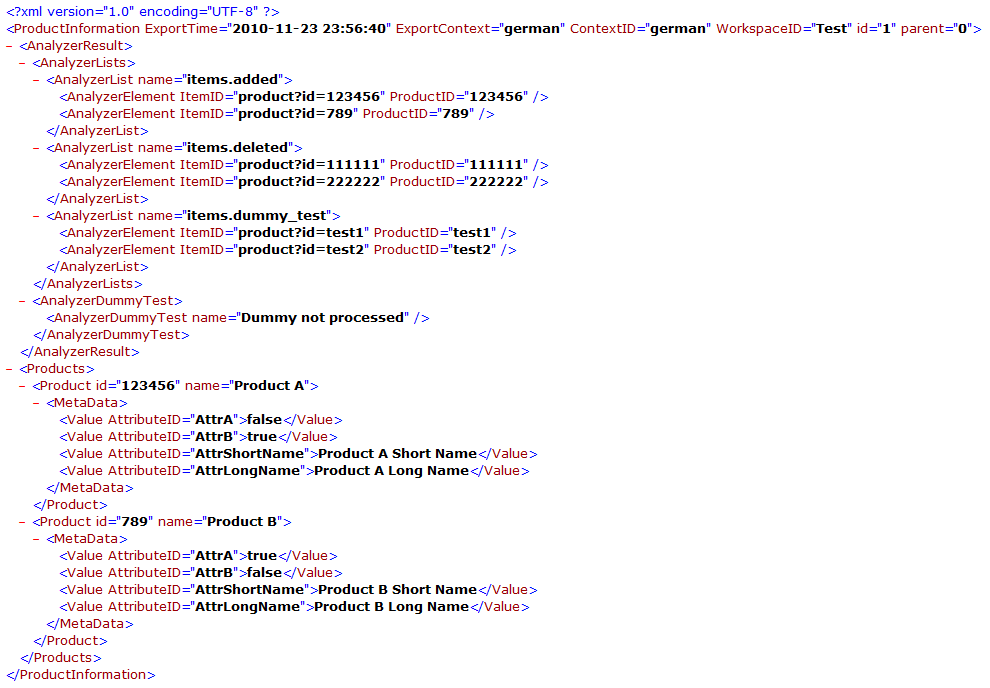
\includegraphics[width=1\linewidth]{imagenes/capitulo3/1*kwUlHDYmt_TaWK7ZefEE8Q}
	\caption{Ejemplo de XML}
	\label{fig:1kwulhdymttawk7zefee8q}
\end{figure}

\textbf{XML (\textit{Extensible Markup Language})} es un lenguaje de marcas, derivado de SGML\footnote{SGML (\textit{Standard Generalized Markup Language}) es un lenguaje para marcar y describir documentos con independencia total del hardware y software utilizados.}, pensado para ser utilizado en el entorno Web y para ser usado en la descripción sintáctica de los recursos, es decir, es la herramienta utilizada para estructurar y presentar los contenidos Web (figura \ref{fig:1kwulhdymttawk7zefee8q}). No obstante, ofrece una capacidad limitada para expresar semántica (no tiene etiquetas predefinidas), por lo que es necesario utilizar lenguajes que permitan imponer restricciones semánticas para descripciones completas \cite{aplicacion}.




%Por tanto, XML responde a la necesidad de representar sintácticamente el modelo planteado por RDF para archivos legibles por ordenador.

% Por eso, se entiende que RDF es a la Semántica lo que XML es a la Sintaxis. Gracias a RDF se expresan afirmaciones y mediante su lenguaje de base XML se define la estructura de tales afirmaciones. Por tanto, XML responde a la necesidad de representar sintácticamente el modelo planteado por RDF para archivos legibles por ordenador.


%Para la descripción sintáctica de los recursos se utiliza XML y XML-Schema como estándares de base, pero es necesario utilizar lenguajes que permitan imponer restricciones semánticas para descripciones completas.

% Originalmente fue diseñado para enfrentar los desafíos de la publicación electrónica a gran escala, XML también desempeña un papel cada vez más importante en el intercambio de una amplia variedad de datos en la Web y en otros lugares.

%Esta página describe el trabajo que se está realizando en W3C dentro de la Actividad XML y cómo está estructurado. El trabajo en el W3C se lleva a cabo en grupos de trabajo. Los grupos de trabajo dentro de la actividad XML se enumeran a continuación, junto con enlaces a sus páginas web individuales.

%Puede encontrar y descargar especificaciones técnicas formales aquí, porque las publicamos. Este no es un lugar para encontrar tutoriales, productos, cursos, libros u otra información relacionada con XML. Hay algunos enlaces a continuación que pueden ayudarlo a encontrar dichos recursos.

%Encontrará enlaces a Recomendaciones del W3C, Recomendaciones propuestas, Borradores de trabajo, conjuntos de pruebas de conformidad y otros documentos en las páginas de cada Grupo de trabajo. Cada documento también contiene direcciones de correo electrónico que puede usar para enviar comentarios o preguntas, por ejemplo, si ha estado escribiendo software para implementarlos y ha encontrado problemas o errores.


%Pero RDF no deja de ser un marco abstracto para describir recursos que requiere de una sintaxis concreta para expresar el conocimiento y transferirlo. De todas las formas sintácticas definidas para la formulación escrita de RDF, la más extendida es, sin lugar a dudas, la basada en XML (Extensible MarkUp Language), un metalenguaje surgido en 1998 bajo los auspicios del W3C. Se trata de un lenguaje de marcas, derivado de SGML, específicamente pensado para ser utilizado en el entorno web.\\


%XML es la herramienta utilizada para estructurar y presentar los contenidos web. Sin embargo, ofrece una capacidad limitada para expresar semántica. Por eso, se entiende que RDF es a la Semántica lo que XML es a la Sintaxis. Gracias a RDF se expresan afirmaciones y mediante su lenguaje de base XML se define la estructura de tales afirmaciones. Por tanto, XML responde a la necesidad de representar sintácticamente el modelo planteado por RDF para archivos legibles por ordenador.


\subsection{RDF} % Resource Description Framework (RDF)

% libro
% w3c
\textbf{RDF} (\textit{Resource Description Framework}) es una familia de especificaciones W3C originalmente diseñada como un modelo de datos de metadatos (datos sobre datos) extendida de XML, pero no es estrictamente un formato XML, y tampoco se trata solo de metadatos. Es un método general para descomponer cualquier tipo de conocimiento en piezas pequeñas, con algunas reglas sobre la semántica o el significado de esas piezas \cite{libro-gis}. Es el estándar más popular y extendido en la comunidad Web; proporciona un entorno para expresar la información de un recurso Web de tal forma que pueda ser intercambiada entre aplicaciones sin pérdida de significado, es decir, es una manera de darle la información desmenuzada al ordenador para que la entienda e identifique cada parte de la sentencia esté en el orden que esté \cite{aplicacion}. \\

La estructura central del RDF es un conjunto de triples (tripletas), que se conoce como grafo RDF y que consta de tres componentes, en donde cada miembro puede ser una referencia a un símbolo (generalmente representado por un URI), que tiene un significado bien definido \cite{web-semantica-w3c}. La figura \ref{fig:tripleta} ilustra los tres componentes de un grafo RDF, y la figura \ref{fig:ejemploRDF} muestra un ejemplo.


\begin{enumerate}
	\item \textbf{Sujeto}: es el recurso, es decir, todo aquello que puede ser descrito.
	\item \textbf{Predicado}: introduce la propiedad que va a detallarse sobre el recurso.
	\item \textbf{Objeto}: es el valor de dicha propiedad.
\end{enumerate}

\begin{figure}[H]
	\centering
	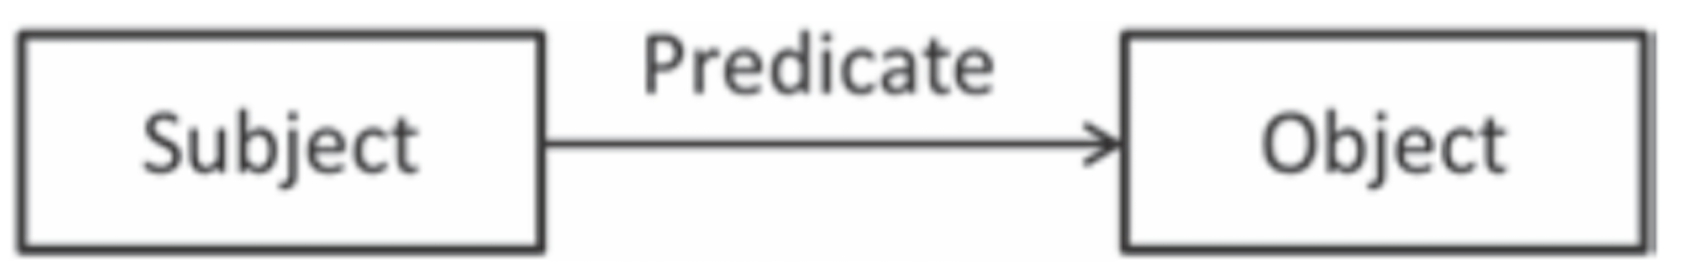
\includegraphics[width=0.53\linewidth]{imagenes/capitulo3/tripleta1}
	\caption{Estructura de un grafo RDF}
	\label{fig:tripleta}
\end{figure}


%en donde el sujeto y el objeto representan los dos recursos relacionados y el predicado representa la relación entre los dos recursos.

\begin{figure}[H]
	\centering
	\begin{subfigure}[h]{0.75\textwidth} 
		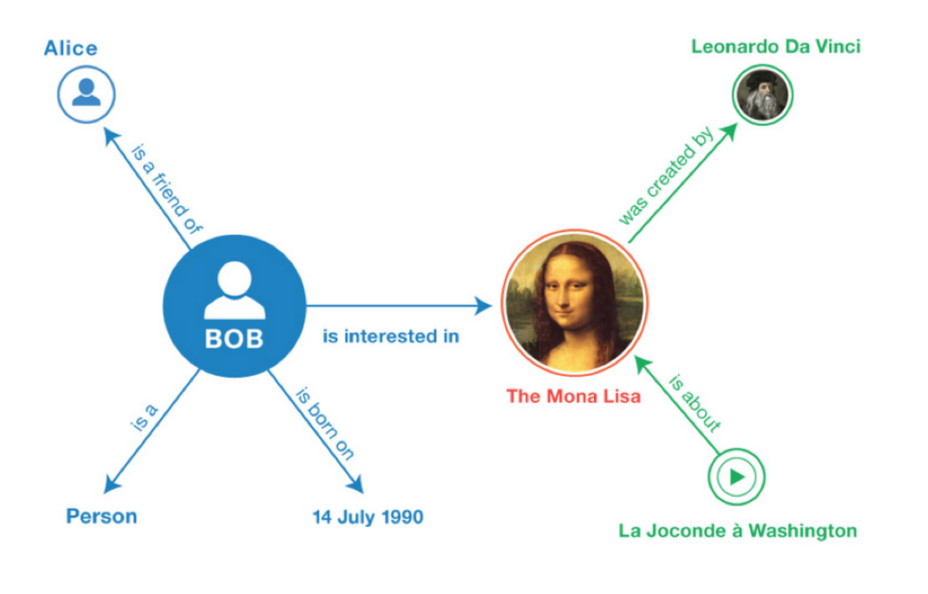
\includegraphics[width=\textwidth]{imagenes/capitulo3/grafoRDF}
		\caption{Grafo RDF}
	\end{subfigure}       
	\begin{subfigure}[h]{0.79\textwidth} 
		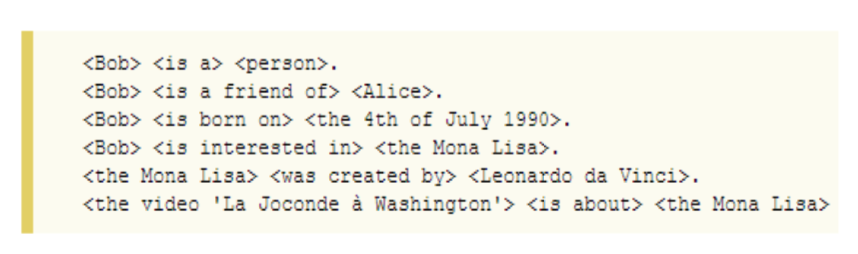
\includegraphics[width=\textwidth]{imagenes/capitulo3/ejemploRDF}
		\caption{Ejemplo RDF Tripleta}
	\end{subfigure}
	\caption{Ejemplo de grafo RDF \cite{aplicacion}}
	\label{fig:ejemploRDF}
\end{figure}

Básicamente RDF es un conjunto de declaraciones que definen clases y propiedades de los recursos. En la tabla \ref{tabla-rdf1} y \ref{tabla-rdf2} se muestra el vocabulario empleado por RDF \cite{tesis-otro}:

\begin{table}[H]
	\caption{Clases del vocabulario RDF}
	\label{tabla-rdf1}
		\centering
	\begin{tabular}{|
			>{\columncolor[HTML]{FFFFFF}}l |m{9cm}|}
		\hline
		\cellcolor[HTML]{EFEFEF}\textbf{CLASE} & \cellcolor[HTML]{EFEFEF} \textbf{DESCRIPCIÓN}\\ \hline
		\texttt{rdf:XMLLiteral}                         & La clase de los valores literales de los valores literales XML                         \\ \hline
		\texttt{rdf:Property}                         &  La clase de las propiedades RDF
		\\ \hline
		\texttt{rdf:Statement}                         &    La clase de las declaraciones RDF
		\\ \hline
		\texttt{rdf:Bag}                         &    La clase de los contenedores desordenados
		\\ \hline
		\texttt{rdf:Seq}                         &    La clase de los contenedores ordenados                      \\ \hline
		\texttt{rdf:Alt}                         &     La clase de los contenedores de alternativas                     \\ \hline
		\texttt{rdf:List}                         &  La clase de las listas RDF                        \\ \hline
	\end{tabular}
	
\end{table}

\begin{table}[H]
	\caption{Propiedades del vocabulario RDF}
	\label{tabla-rdf2}
		\centering
	\begin{tabular}{|
			>{\columncolor[HTML]{FFFFFF}}l |m{9cm}|}
		\hline
		\cellcolor[HTML]{EFEFEF}\textbf{PROPIEDAD} & \cellcolor[HTML]{EFEFEF} \textbf{DESCRIPCIÓN}\\ \hline
		\texttt{rdf:type}                         &      El sujeto es una instancia de una clase                    \\ \hline
		\texttt{rdf:first}                         &   El primer item en la lista RDF del sujeto                       \\ \hline
		\texttt{rdf:rest}                         &        El resto de la lista RDF del sujeto despúes del primer item                  \\ \hline
		\texttt{rdf:value}                         &    Propiedad idiomática usada para valores estructurados                       \\ \hline
		\texttt{rdf:subject}                         &     El sujeto de la declaración RDF del sujeto                     \\ \hline
		\texttt{rdf:predicate }                         &      El predicado de la declaración RDF del sujeto                    \\ \hline
		\texttt{rdf:object}                         &        El objeto de la declaración RDF del sujeto                  \\ \hline
	\end{tabular}
\end{table}

En la figura \ref{fig:ejemplo-rdf} podemos ver un ejemplo de RDF a partir del vocabulario que acabamos de ver en las tablas anteriores.

\begin{figure}[H]
	\centering
	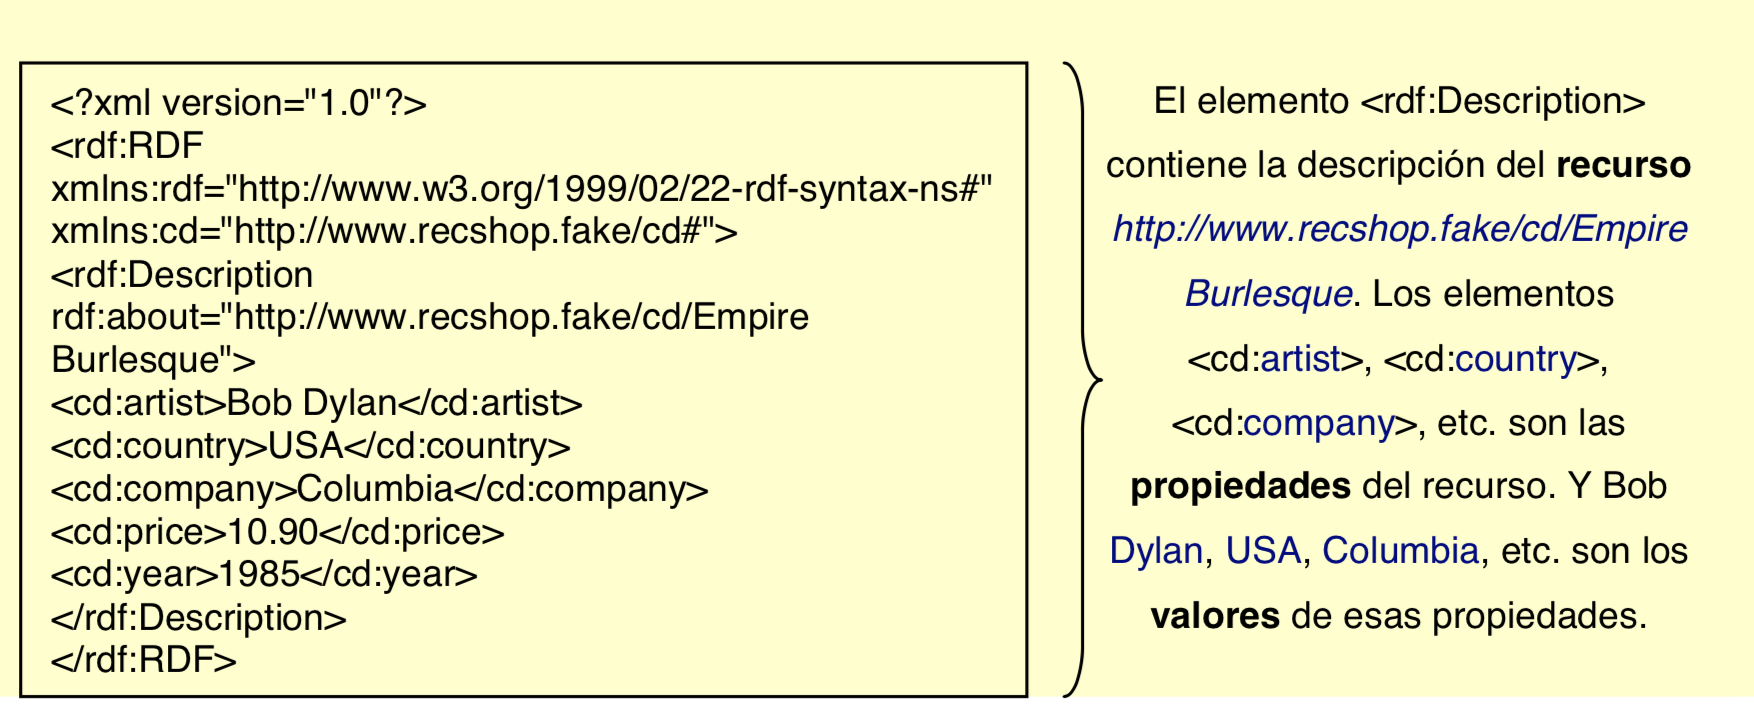
\includegraphics[width=1\linewidth]{imagenes/capitulo3/ejemplo-RDF}
	\caption{Descripción de un recurso musical en RDF \cite{web-semantica-w3c}}
	\label{fig:ejemplo-rdf}
\end{figure}

\begin{figure}[H]
	\centering
	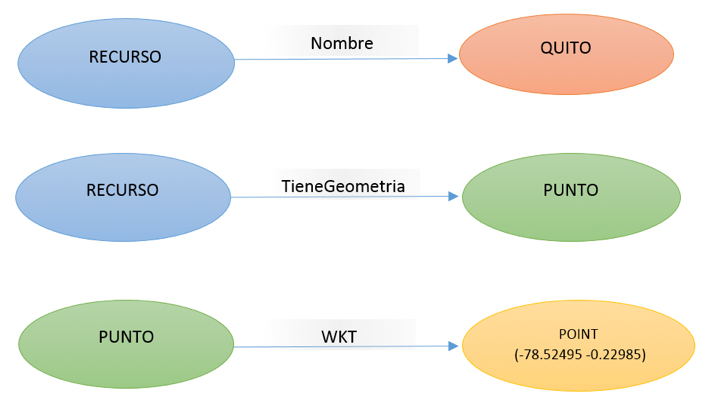
\includegraphics[width=0.75\linewidth]{imagenes/capitulo3/Imagen1}
	\caption{Ejemplo de tripletas \cite{coursera}}
	\label{fig:imagen1}
\end{figure}


En la figura \ref{fig:imagen1} se muestra otro ejemplo de tripletas que indican la relación entre un recurso, nombre del recurso y geometría, es decir, en este caso el sujeto es el \textit{Recurso} que tiene la propiedad \textit{Nombre} cuyo valor es \textit{Quito}, además \textit{Recurso} tiene la propiedad \textit{Geometría} cuyo valor es \textit{Punto} y finalmente se indica que el sujeto \textit{Punto}, tiene la propiedad \textit{WKT} que indica el formato de la geometría, cuyo valor es \textit{POINT(-78.52495 -0.22985)} \cite{coursera}. \\


Por tanto, se entiende que RDF es a la semántica lo que XML es a la sintaxis, ya que XML responde a la necesidad de representar sintácticamente el modelo planteado por RDF para archivos entendibles por ordenador \cite{web-semantica-w3c}.


\subsection{RDF Schema}

\textbf{Esquema RDF} o \textbf{RDFS} \textbf{(RDF Schema)} es una extensión semántica que enriquece a RDF. Es un vocabulario que permite definir un primer sistema de jerarquías entre las clases de recursos, especificando las propiedades y relaciones admitidas entre ellas, es decir, permite a los usuarios definir características semánticas de los datos RDF y comprobar las restricciones semánticas \cite{web-semantica-w3c, libro-gis, aplicacion}. Igual que se han definido para RDF, existe un vocabulario empleado por RDFS (tablas \ref{tabla-rdfs1} y \ref{tabla-rdfs2}) \cite{tesis-otro}.\\

Sin embargo, RDFS tiene limitaciones al carecer de expresividad para: información negativa (las mujeres no son hombres), cuantificadores (para que alguien sea considerado madre debe tener al menos un hijo), cardinalidad (un buen estudiante tiene que tener aprobadas más de 4 asignaturas) y no permite atributos de propiedades (transitiva, simétrica, inversa). Por todo esto y más, no se considera lo bastante completo para describir los recursos de la Web con el detalle necesario, pero se utiliza porque se puede emplear en muchos dominios y actuar de puente entre vocabularios \cite{aplicacion}.

%Junto al RDF, se usa RDFS (RDF Schema) para definir las propiedades de los recursos y los tipos de recursos que son descritos. Es un mecanismo necesario para detallar cada elemento, especificar un vocabulario para definir las clases y propiedades, restringir las posibles combinaciones de clases y relaciones, y detectar violaciones de estas restricciones. Mientras un XML Schema puede ser utilizado para validar la sintaxis de un RDF/XML, un RDF Schema permite comprobar las restricciones semánticas.

\begin{table}[H]
	\caption{Clases del vocabulario RDFS}
	\label{tabla-rdfs1}
	\centering
	\begin{tabular}{|
			>{\columncolor[HTML]{FFFFFF}}l |m{8.9cm}|}
		\hline
		\cellcolor[HTML]{EFEFEF}\textbf{CLASE} & \cellcolor[HTML]{EFEFEF} \textbf{DESCRIPCIÓN}\\ \hline
		\texttt{rdfs:Resource}                         &        La clase de recurso, cada uno
		\\ \hline
		\texttt{rdfs:Literal}                         &        La clase del valor literal, por ejemplo, cadenas de texto y números enteros                  \\ \hline
		\texttt{rdfs:Class}                         &        La clase de las clases
		\\ \hline
		\texttt{rdfs:Datatype}                         &    La clase de los tipos de datos RDF                      \\ \hline
		\texttt{rdfs:Container}                         &   La clase de los contenedores RDF                       \\ \hline
	\end{tabular}
\end{table}

\begin{table}[H]
	\caption{Propiedades del vocabulario RDF}
	\label{tabla-rdfs2}
	\centering
	\begin{tabular}{|
			>{\columncolor[HTML]{FFFFFF}}l |m{8cm}|}
		\hline
		\cellcolor[HTML]{EFEFEF}\textbf{PROPIEDAD} & \cellcolor[HTML]{EFEFEF} \textbf{DESCRIPCIÓN}\\ \hline
		\textbf{rdfs:subClassOf}                         &         El sujeto es una subclase de una clase                 \\ \hline
		\textbf{rdfs:subPropertyOf}                         &     El sujeto es una subpropiedad de una propiedad                     \\ \hline
		\textbf{rdfs:domain}                         &           Un dominio de la propiedad del sujeto               \\ \hline
		\textbf{rdfs:range}                         &        Un rango de la propiedad del sujeto                  \\ \hline
		\textbf{rdfs:label}                         &        Un nombre para el sujeto legible por seres humanos                   \\ \hline
		\textbf{rdfs:comment}                         &        Una descripción del recurso sujeto                  \\ \hline
		\textbf{rdfs:member}                         &        Un miembro del recurso sujeto                  \\ \hline
		\textbf{rdfs:seeAlso}                         &              Más información sobre el recurso sujeto            \\ \hline
		\textbf{rdfs:isDefinedBy}                         &       La definición del recurso sujeto. 
		\\ \hline
	\end{tabular}
\end{table}



\subsection{Ontología} % Web Ontology Language (OWL)

% tesis
La \textbf{ontología} es un concepto filosófico adoptado por la Informática, que parte de la metafísica y que trata del ser en general y de sus propiedades trascendentales \cite{apuntes-clase-jose}. Se trata de un esquema conceptual que define los términos a utilizar para describir y representar un área de conocimiento dado, con el objetivo de facilitar la comunicación entre diferentes entidades, es decir, codifican el conocimiento de un dominio y de esta manera hacen el conocimiento reutilizable \cite{tesis}. Así, definen de forma estándar y consensuada un vocabulario de conceptos como las relaciones entre ellos dentro de un área concreta del conocimiento, formando redes jerárquicas semánticas y recogiendo reglas lógicas y restricciones para hacer comprender a las máquinas los conceptos de un determinado campo. Por ejemplo, \textit{una ontología de arte establece que todos los escultores son artistas pero no todos los artistas son escultores} \cite{web-semantica-w3c}. En una ontología nos podemos encontrar \cite{aplicacion, apuntes-clase-jose}:

\begin{itemize}
	\item \textbf{Conceptos}: sujetos básicos que se intentan formalizar sobre cualquier tipo de clase. En una ontología de deportes, cada clase sería un deporte: natación, baloncesto, tenis.
	
	\item  \textbf{Relaciones}: enlace entre los conceptos, cómo interactúan los conceptos del dominio (subclase-de, parte-de).
	
	\item \textbf{Propiedades}: definen características o atributos de los conceptos.
	
	\item \textbf{Instancias}: objetos particulares de un concepto.
		
	\item \textbf{Funciones}: tipo de relación en la que el elemento es el resultado de la aplicación directa de una operación sobre varios conceptos de la ontología.
		
	\item \textbf{Axiomas}: teoremas que se declaran sobre relaciones, y que deberán cumplir los elementos de la ontología. Es la clave de la inferencia de conocimiento. Por ejemplo, \textit{si A conoce B, B conoce A}.
	
	\item \textbf{Constantes}: permiten representar valores primitivos como cadenas de caracteres o valores numéricos
	
	\item \textbf{Restricciones}: descripciones sobre qué debe cumplirse para que un axioma sea cierto.
	
\end{itemize}

%Las ontologías pueden ser modeladas con diferentes técnicas de modelado de conocimiento y a su vez implementadas con diferentes lenguajes. Algunas de las técnicas de modelado son utilizando: marcos y lógica de primer orden, lógica descriptiva, UML o bien diagramas Entidad-Relación. Entre los lenguajes de implementación, el W3C recomienda RDF y OWL.

Una vez visto el concepto de ontología y su posible aplicación a la Web Semántica, es posible pasar a explicar OWL.

\subsubsection{OWL}

\textbf{OWL} \textbf{(\textit{Lenguaje de Ontologías Web})} es un lenguaje ontológico para la Web Semántica con significado formalmente definido, sirve para definir ontologías Web estructuradas y provee de más vocabulario para la descripción de propiedades y clases, por ejemplo: relaciones entre clases, cardinalidad, equivalencia y características de propiedades (figura \ref{fig:ejemplo-owl}). Realmente, OWL es una extensión del lenguaje RDF y emplea tripletas de RDF (figura \ref{fig:nomenclatura}), aunque es un lenguaje con más poder expresivo \cite{aplicacion}.

\begin{figure}[H]
	\centering
	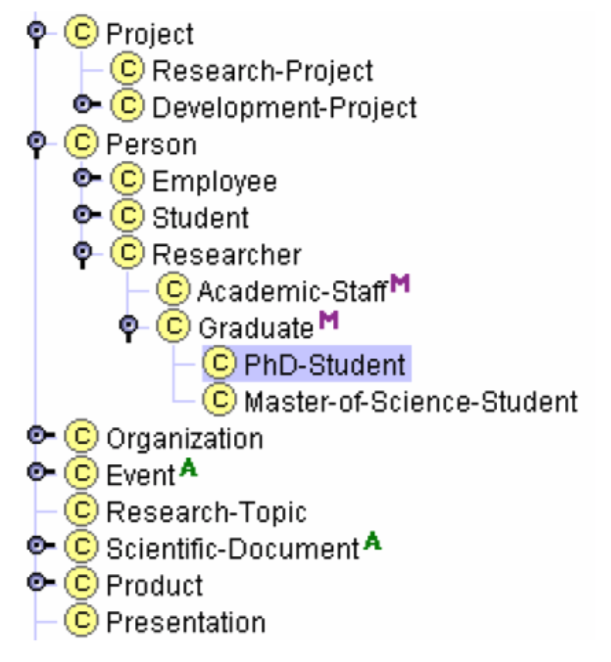
\includegraphics[width=0.51\linewidth]{imagenes/capitulo3/ejemplo-owl}
	\caption{Ejemplo de una ontología \cite{apuntes-clase-jose}}
	\label{fig:ejemplo-owl}
\end{figure}

\begin{figure}[H]
	\centering
	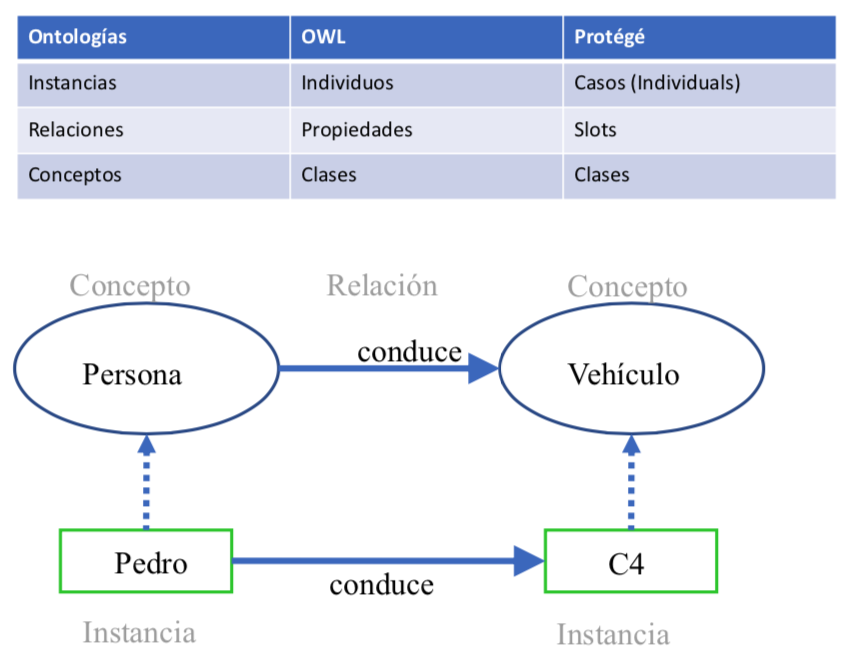
\includegraphics[width=0.63\linewidth]{imagenes/capitulo3/nomenclatura}
	\caption{Nomenclatura básica ontología OWL \cite{apuntes-clase-jose}}
	\label{fig:nomenclatura}
\end{figure}

%OWL puede formularse en RDF, que ofrece la base adecuada para desarrollar ontologías, y mejora la capacidad expresiva de RDFS. Al construirse sobre RDF, las ontologías OWL podrán ser distribuidas en diferentes sistemas y ser compatibles con otros estándares web.\\
En Octubre de 2009 nació \textit{OWL 2 Web Ontology Language} como recomendación del W3C para la edición de ontologías, extensión de la primera versión OWL 1 publicada en 2004. OWL 1 proporciona tres lenguajes, cada uno con nivel de expresividad mayor que el anterior, diseñados para ser usados por comunidades específicas de desarrolladores y usuarios \cite{owl-tipos}. En OWL 2 se definen tres nuevos perfiles y se proporcionan tres sublenguajes que ofrecen ventajas en escenarios particulares, todos más restrictivos que OWL DL y cada uno con diferentes aspectos expresivos a cambio de diferentes beneficios computacionales y/o de implementación \cite{aplicacion}. 

\begin{itemize}
	\item \textbf{OWL Lite}: diseñado para aquellos usuarios que necesitan principalmente creación de jerarquías y restricciones simples.
	
	\item \textbf{OWL DL}: es el lenguaje habitual de ontologías diseñado para aquellos usuarios que quieren la máxima expresividad conservando completitud computacional, es decir, está basado en lógica descriptiva y proporciona la máxima capacidad de expresión para garantizar computabilidad y decidibilidad (todas las conclusiones pueden ser deducidas y todos los cálculos se realizan en un tiempo finito).
	
	\item \textbf{OWL Full}: diseñado para aquellos usuarios que quieren máxima expresividad y libertad sintáctica de RDF sin garantías computacionales, es decir, permite expresividad de segundo orden, pero sin decidibilidad (no hay garantía computacional).
\end{itemize}

Por otro lado, las ontologías deben de cumplir unas características: sintaxis bien definida, semántica específica, expresividad, fácilmente traducible entre los lenguajes ontológicos y eficiencia para realizar razonamientos \cite{apuntes-clase-jose}.\\

No obstante, escribir en lenguajes como RDF y OWL resultan sumamente difícil y propensos a errores. Afortunadamente, existen en el mercado entornos gráficos para visualizar y construir ontologías de forma más razonable, como \textbf{Protegé}, software desarrollado por la Universidad de Stanford. Permite editar ontologías con una interfaz sencilla y en un entorno de menús, botones, cuadros de diálogo o representaciones gráficas fáciles de usar, tan importantes para una tarea con tanta de abstracción y síntesis.

\subsection{Lenguajes de consulta}


Por último, nos queda presentar dos lenguajes de consulta semántica: SPARQL, estándar ampliamente utilizado para consultar datos RDF y GeoSPARQL, extensión de SPARQL que admite operaciones geoespaciales.


\subsubsection{SPARQL}

% dbpedia, que es la representación en RDF en wikipedia la dbpedia en español


% COURSERA: La Web Semántica: Herramientas para la publicación y extracción efectiva de información en la Web
%Hola, bienvenido a nuestro curso sobre la web semántica, en este video comenzaremos a ver algunas de la nociones básicas sobre el lenguaje de consulta SPARQL, en particular veremos la nociones de variables y patrones en SPARQL. Como ya hemos mencionado en los videos anteriores en la web existe una multitud de base de datos de RDF, por ejemplo dbpedia, que es la representación en RDF en wikipedia la dbpedia en español y IMDB que es una base de películas, etcétera. Muchas de estas bases RDF permiten acceder a sus datos utilizando el lenguaje de consulta SPARQL, recuerde que SPARQL es un lenguaje que nos permite escribir de manera precisa la información que queremos extraer y que es procesable por un computador, vale decir un computador puede de manera automática construir las respuestas de una consulta SPARQL. Entonces en esta base de datos RDF nos permiten utilizar este lenguaje SPARQL y la forma de hacerlo es a través de lo que es llamado un SPARQL endpoint, que es un servicio web donde uno puede colocar este tipos de consultas. En esta transparencia puede ver la dirección de dos de estos servicios web, la primera de ellas es el SPARQL endpoint de dbpedia que es dbpedia.org/sparql, la segunda es el SPARQL endpoint de dbpedia en español.

%En esta transparencia usted puede ver este grafo RDF escrito en un archivo como una secuencia de triples, recuerde cuando teníamos una secuencia de triples en primer lugar especificamos los prefijos que vamos a utilizar en los URIs, recuerden que estos prefijos son utilizados para simplificar la notación que tenemos en estos URIs Una vez que hemos escrito estos prefijos en este caso tenemos dbpprop, dbpedia-owl y dbpedia construimos nuestros triples en esta caso tenemos cuatro triples el primero de ellos es dbpedia:Santiago rdf:type y dbpedia-owl:place, en este triple estamos diciendo que Santiago es de tipo lugar. En esta transparencia usted puede ver un grafo en la dbpedia con datos sobre lugares, esto simplemente es parte del grafo anterior donde decíamos bueno dbpedia:Santiago es de tipo lugar, que se encuentra en Chile y que su nombre oficial es Santiago. En esta transparencia usted tambien puede ver una consulta SPARQL y a continuación mostraremos las distintas partes de esta consulta, en primer lugar tenemos el encabezado de la consulta que puede ver en amarillo, este encabezado se puede distinguir a través de la palabra SELECT. En segundo lugar tenemos el patrón de la consulta que en este caso también esta desatascado en amarillo y que se encuentra dentro de la cláusula where. Es importante destacar que el patrón sigue la estructura sujeto, predicado, objeto. Por ejemplo en este caso tenemos un patrón de nuevo podemos ver este patrón en amarillo en el cual tenemos dos triples, en el primer triple ?X dbpprop:officialName ?name tenemos como sujeto a X, como predicado a dbprop:officialName y como objeto a name. En el segundo triple tenemos como sujeto a X, como predicado a rdf:type y como objeto a dbpedia-owl:Place. También es importante destacar que en este patrón tenemos variables y tenemos URIs, cada variable en una consulta SPARQL comienza con el signo de pregunta. En este caso entonces, tenemos como variables a signo de pregunta X y signo de pregunta name. También en una consulta SPARQL podemos tener URIs y en estos URIs utilizamos la notación usual, por ejemplo en esta consulta tenemos el URI dbpprop:officialName, en este caso estamos usando el prefijo dbpprop: ¿Cómo se calcula la respuesta a una consulta SPARQL? Bueno, en el patrón remplazamos cada variable por un URI o por un literal, y lo que es importante es que los triples resultantes de este remplazo debe estar en el grafo RDF. por ejemplo, en este caso podemos remplazar como he mostrado en la figura la variable X por dbpedia:Santiago y la variable name por Santiago. Si hacemos este remplazo entonces en el primer triple vamos a obtener el triple de dbpedia:Santiago, dbpprop:officialName Santiago que es un type que esta en el grafo RDF como es marcado en rojo. Lo que es importante en este caso es que tenemos que hacer el mismo remplazo en el segundo triple, y en este caso vamos a obtener el triple dbpedia:Santiago rdf:type, dbpedia-owl:place que tambien esta en nuestro grafo RDF. Por lo tanto en este caso tenemos un remplazo exitoso. ¿Para qué sirve el encabezado de una consulta SPARQL? El encabezado nos indica en este caso tenemos SELECT ?name por lo tanto nos está indicando que vamos a retornar los valores que hemos dado a la variable name, en este caso Santiago vale decir, esta consulta nos permite encontrar todos los nombres oficiales de los lugares que tenemos en dbpedia.

\textbf{SPARQL} es un lenguaje estandarizado por la W3C clave para el desarrollo de la Web Semántica que permite escribir de manera precisa la información que queremos extraer, es decir, es una especificación que ofrece un lenguaje y protocolos para consultar y manipular RDF \cite{tesis-otro}. En la figura \ref{fig:sparql}, podemos encontrar una consulta básica de selección SPARQL y comprobar que la estructura de este lenguaje se asemeja a SQL. Entre las características de SPARQL, resaltan (tabla \ref{carac-sparql}): 

\begin{table}[H]
	\caption{Características de SPARQL}
	\label{carac-sparql}
	\centering
	\begin{tabular}{|l|}
		\hline
		 Lenguaje de consulta \\ \hline
		 Formato XML, JSON, CSV y TSV  para resultados en una consulta \\ \hline
Actualización de grafos RDF	\\ \hline
	Protocolo para RDF	\\ \hline
	Descubrir información acerca de la información  almacenada (\textit{dataset})	\\ \hline
	 Manejo de grafos mediante el protocolo HTTP 	\\ \hline
	\end{tabular}
\end{table}

\begin{figure}[H]
	\centering
	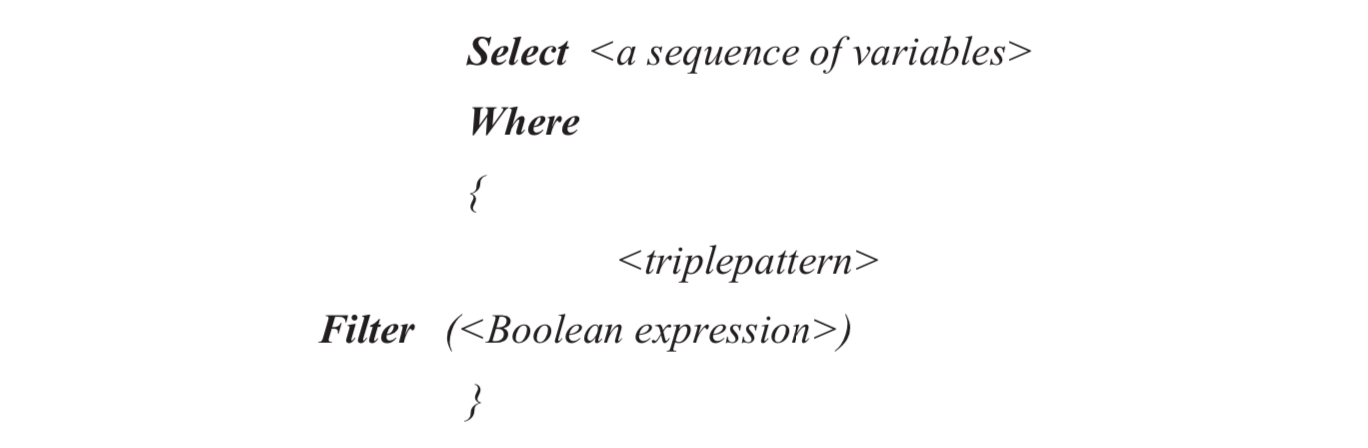
\includegraphics[width=1.1\linewidth]{imagenes/capitulo3/sparql}
	\caption{Estructura de una consulta en SPARQL}
	\label{fig:sparql}
\end{figure}

Los resultados de una consulta están restringidos por una sección \texttt{WHERE}, que proporciona el patrón de gráfico básico para que coincida con el gráfico de datos. El patrón gráfico consiste en un conjunto de triples, que forman un gráfico, donde un elemento de un triple puede ser un URI de un recurso, un valor de datos (en el caso del objeto triple) o una variable. Una variable tiene el prefijo con el signo de interrogación y puede aparecer en la sección \texttt{SELECT} (la variable de salida). La sección \texttt{WHERE} también puede contener cláusulas \texttt{FILTER}, que filtran, por ejemplo cadena y valores numéricos usando varias funciones (predicados) \cite{tesis-otro}.\\

Un ejemplo simple de una consulta SELECT se encuentra en la figura \ref{fig:ejemplo-sparql}, en donde se quieren obtener de la Dbpedia, ingenieros que residen en ciudades con una población de más de 10000000 habitantes. En la figura \ref{fig:salida-sparql} se puede observar la salida a dicha consulta \cite{tesis-otro}.

\begin{figure}[H]
	\centering
	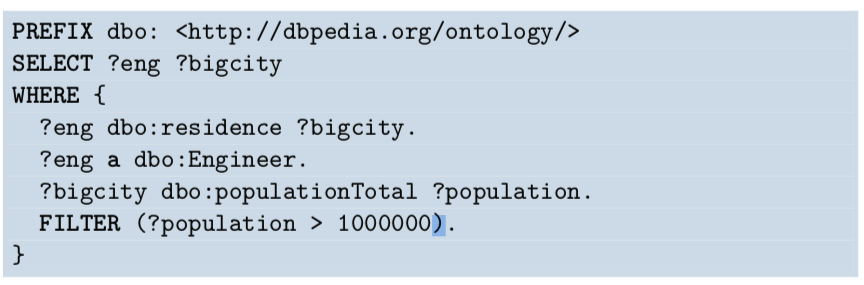
\includegraphics[width=0.9\linewidth]{imagenes/capitulo3/ejemplo-sparql}
	\caption{Ejemplo de consulta de SPARQL \cite{tesis-otro}}
	\label{fig:ejemplo-sparql}
\end{figure}

\begin{figure}[H]
	\centering
	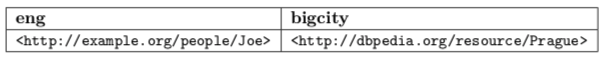
\includegraphics[width=0.9\linewidth]{imagenes/capitulo3/salida-sparql}
	\caption{Respuesta a la salida de la consulta de la figura \ref{fig:ejemplo-sparql}}
	\label{fig:salida-sparql}
\end{figure}


%En la figura 2.3 se muestra un ejemplo de consulta SPARQL, haciendo referencia a las tripletas de la figura 2.2, se observa la estructura de la consulta para obtener los datos deseados como el Nombre del recurso, tipo de geometría y la geometría en formato WKT. Lo que se encuentra en el recuadro de color verde permite identificar el recurso, en este caso “Quito”, posteriormente en el recuadro de color rojo se observa la parte de la consulta que permite obtener el tipo de geometría del recurso “Quito” y finalmente en el recuadro de color azul se encuentra la parte de la consulta que permite obtener la geometría en formato WKT del recurso “Quito”, tambíen se muestra el resultado generado por la consulta SPARQL. 

Como hemos comentado anteriormente, la herramienta Protegé nos permite construir contologías de manera más sencilla y rápida, sin embargo, también ofrece herramientas para realizar consultas con SPARQL. No obstante, aunque SPARQL sea un lenguaje ampliamente utilizado para consultar ontologías RDF, carece de las construcciones necesarias para consultar datos espaciales. Afortunadamente, disponemos del estándar: GeoSPARQL.

\subsubsection{GeoSPARQL}

% tesis
% libro
\textbf{GeoSPARQL} es un estándar establecido por \textit{Open Geoespatial Consortium} (OGC). Es una extensión del lenguaje de consulta SPARQL para recuperar información geoespacial de conjuntos de datos RDF en la Web Semántica \cite{libro-gis}. Entre sus características podemos encontrar \cite{ogc-geo}: 

\begin{itemize}
	\item Vocabulario RDF/OWL para representar información geoespacial.
	\item Funciones extensión a SPARQL para cálculos espaciales.
	\item Conjunto básico de clases, propiedades y tipo de datos que son utilizados para construir patrones de consulta (figura \ref{fig:geosparql}). 
\end{itemize}

\begin{figure}[H]
	\centering
	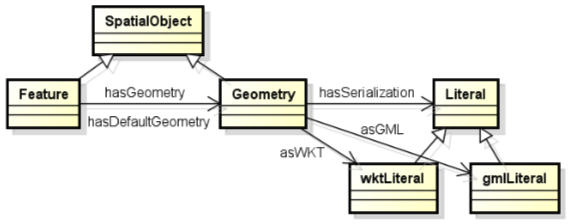
\includegraphics[width=0.83\linewidth]{imagenes/capitulo3/geosparql}
	\caption{Clases y propiedades básicas de GeoSPARQL}
	\label{fig:geosparql}
\end{figure}

GeoSPARQL no define un vocabulario completo para representar información espacial, sino que define un conjunto central de clases, propiedades y tipos de datos que se pueden utilizar para construir patrones de consulta (figura \ref{fig:geosparql}) \cite{ogc-geo}. Es un lenguaje muy enfocado para la comunidad SIG. Por otro lado, para poder hacer uso de este tipo de consultas es necesario aplicar las especificaciones que vienen descritas en la documentación oficial\footnote{\url{https://www.opengeospatial.org/standards/geosparql}}. \\

En la tabla \ref{topo-geosparql} podemos encontrar sus relaciones topológicas, mientras que en la tabla \ref{funciones-geosparql} podemos encontrar funciones de GeoSPARQL que incluyen alternativas de todas las propiedades de relación topológica, aplicadas como funciones en literales de geometría \cite{tesis-otro}. Respecto la geometría permite puntos, líneas y polígonos, como vimos en el capítulo anterior y además la representación de la geometría debe de estar codificada en formato WKT.

\begin{table}[H]
	\caption{Relaciones topológicas con sus significados}
	\label{topo-geosparql}
	\centering
	\begin{tabular}{|l|l|}
		\hline
		\rowcolor[HTML]{EFEFEF} 
		{\textbf{OBJETO}} & { \textbf{DESCRIPCIÓN}} \\ \hline
	\texttt{sfEquals}	&              Espacialmente igual           \\ \hline
	\texttt{sfDisjoint}	&        Disjunto (no puede tocar)                 \\ \hline
	\texttt{sfIntersects}	&     Comparten al menos un punto                    \\ \hline
\texttt{sfTouches} &          Se tocan externamente               \\ \hline
	\texttt{sfWithin}	&      Está dentro (puede tocar el límite)                   \\ \hline
\texttt{sfContains} &             El inverso de \texttt{sfWithin}            \\ \hline
	\texttt{sfOverlaps}	&            Tienen algunos puntos comunes, misma dimensión             \\ \hline
\texttt{sfCrosses} &         Por ejemplo, área cruza la línea                \\ \hline		
	\end{tabular}
\end{table}


\begin{table}[H]
	\caption{Funciones para comparar y manipular geometrías}
	\label{funciones-geosparql}
	\centering
	\begin{tabular}{|l|m{8.6cm}|}
		\hline
		\rowcolor[HTML]{EFEFEF} 
		{\textbf{FUNCIÓN} } & {\textbf{DESCRIPCIÓN}} \\ \hline
\texttt{distance}		&       La distancia de dos literales geométricos medidos en unidades dadas                  \\ \hline
\texttt{buffer} &           Literal de geometría como un literal de entrada con un buffer agregado, dado el radio y las unidades del buffer              \\ \hline
	\texttt{convexHull}	&      El casco convexo de un literal de geometría                   \\ \hline
\texttt{intersection} &          La intersección de dos literales de geometría               \\ \hline
\texttt{union}		&     Unión de dos literales de geometría                    \\ \hline
\texttt{difference} &       La diferencia de dos literales de geometría                  \\ \hline
	\texttt{symDifference}	&      Establecer la diferencia simétrica de dos literales de geometría                  \\ \hline
\texttt{envelope}  &              El cuadro delimitador de un literal de geometría           \\ \hline
\texttt{boundary}		&    El límite de un literal de geometría                     \\ \hline
\texttt{getsrid} &       URI del sistema de referencia espacial de un literal de geometría                  \\ \hline		
	\end{tabular}
\end{table}

En el apartado siguiente, haremos uso de este lenguaje para la obtención de la información geoespacial deseada, centrándonos en varios ejemplos prácticos, y su uso de cara al futuro. Con esto hemos terminado de explicar las tecnologías de la Web Semántica. En la figura \ref{fig:arquitectura2copia} podemos apreciar el recorrido que hemos hecho por las distintas capas que tiene la arquitectura para la Web Semántica. Como el resto de capas no resultan relevantes para nuestro proyecto, se ha obtado por no exponerlas, para así enfocar el presente trabajo en el objetivo planteado al principio del mismo.

\begin{figure}[H]
	\centering
	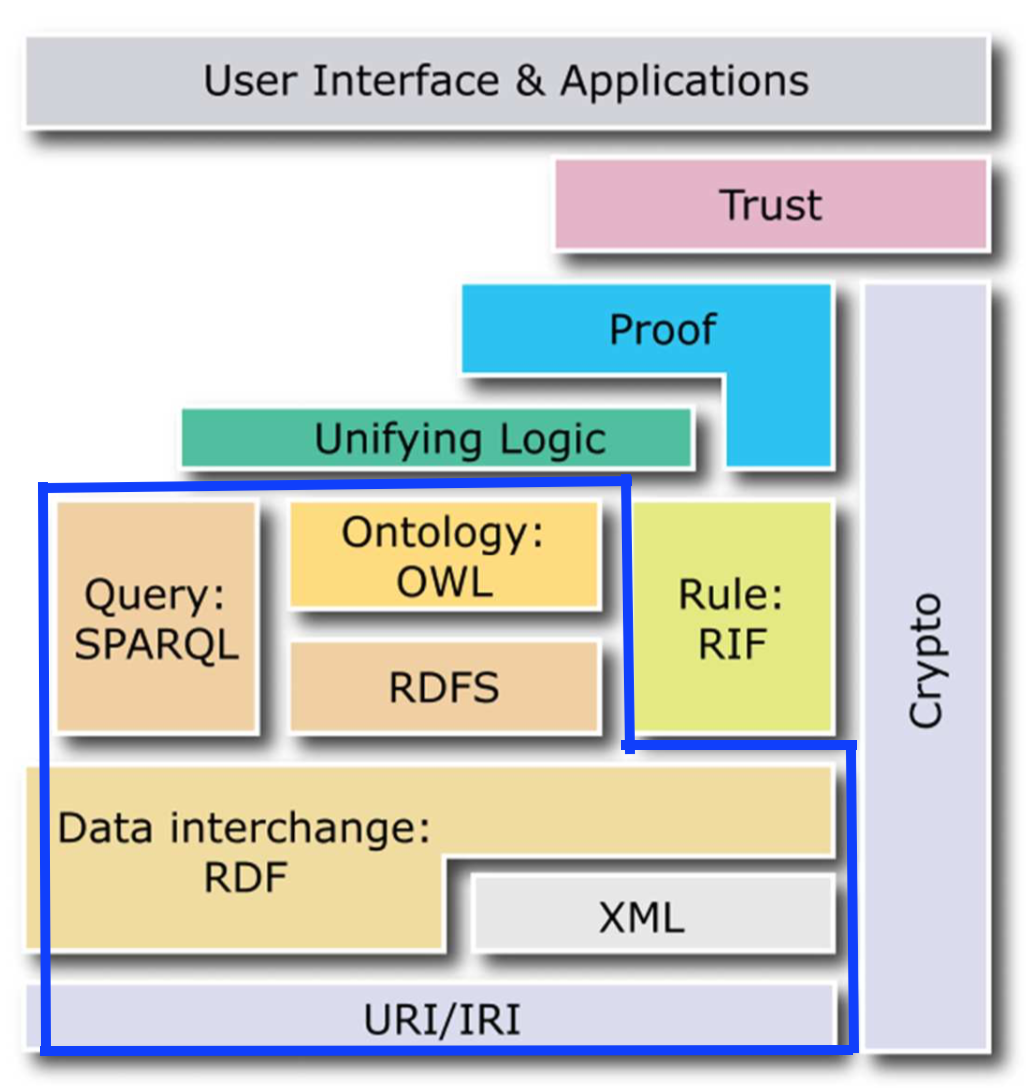
\includegraphics[width=0.48\linewidth]{imagenes/capitulo3/arquitectura2copia}
	\caption{Tecnologías de la Web Semántica explicadas}
	\label{fig:arquitectura2copia}
\end{figure}

\section{¿Qué no es la Web Semántica?}

Una vez expuestos los contenidos que comprenden la Web Semántica, es necesario enfatizar qué no es la Web Semántica, con el objeto de evitar posibles confusiones futuras. Durante el presente trabajo, hemos hablado de que la Web Semántica es una extensión de la actual Web, por tanto diremos que una Web no es Semántica cuando sea diferente a la actual Web y tenga estándares incompatibles con la Web actual \cite{introduccion}. Además, debe seguir cumpliendo las características que conforman la Web, puesto que una Web de navegacioón compleja no transparente y difícil de usar para usuarios, tampoco entraría dentro de lo que llamamos Web Semántica. Además, no todos los navegadores hacen uso de búsquedas semánticas, ya que la mayoría se basan por similtudes con las palabras usadas para la búsqueda sin hacer uso de la interpretación de la información.

\section{Aplicaciones de la Web Semántica}


%Prototipo de un sistema semántico de diagnosis para congestiones de tráfico en carretera desarrollado por IBM (68), donde se presenta un prototipo que analiza de forma semántica y mediante enfoques de inteligencia artificial el histórico de congestiones de trafico para determinar las causas de situaciones inesperadas en casi tiempo real de la situación del trafico en la ciudad de Dublín.
%
%
%Aplicación de la Web Semántica en Trafico
%
%
%Reino Unido (data.gov.uk)
%
%El principal ejemplo encontrado con información de tráfico es el proporcionado desde el apartado transporte de la iniciativa de datos gubernamentales del Reino Unido (58), que permite consultar la información sobre estaciones de tren, aeropuertos y paradas de autobús entre otros, mediante consultas SPARQL.
%Por ejemplo para las estaciones de tren, se pueden lanzar las consultas mediante una interfaz similar a la de la ilustración, obteniendo el listado de las estaciones resultantes en diferentes formatos disponibles (ilustración 19):
%
%Desde data.gob.uk, también se puede acceder a información como los datos de tráfico, eventos planeados y no planeados en (59) pero esta vez en formato XML, siguiendo la estructura propuesta por DATEX II v1.0. El ejemplo de futuros eventos planificados puede consultarse en (60).
%Otra información disponible son los datos relativos a los conteos de tráfico en una región, pero estos sólo están disponibles en CSV o bien en PDF, sin integrar tampoco formatos RDF. Se pueden consultar desde (61).
%
%Estos ejemplos, son interesantes debido al tipo de información que publican, pero es necesario destacar que no se utilizan estándares de Web Semántica en la publicación de los datos, con lo que no se alcanzarían las 4 estrellas de la escala comentada en el apartado 4.2 Linked Data.

%Directorios y catálogos de documentos.
%Openguides.org
%www.dmoz.org
%Redes Sociales. FOAF
%http://www.foaf-project.org/
%Buscadores semánticos.
%http://www.aktors.org/technologies/csaktivespace/

%Buscadores Semánticos: Satisfacer las expectativas de búsqueda de usuarios que requieren resultados precisos.

% http://www.fgcsic.es/lychnos/es_es/articulos/construyendo_una_web_semantica

Los conceptos que acabamos de ver han repercutido en la actualidad, ya que existen diversas aplicaciones que de una forma u otra se basan en tecnologías semánticas para la Web. A continuación, mostramos algunas \cite{cwb}:

\begin{itemize}
	\item % http://www.fgcsic.es/lychnos/es_es/articulos/construyendo_una_web_semantica
	\textbf{Producción científica}: en el campo de la ciencia, la publicación de resultados de la experimentación es fundamental para la comunidad científica. Un ejemplo de ello es el portal \textbf{GoPubMed}\footnote{Actualmente no disponible (\url{https://www.gopubmed.org/})}, que ofrece un buscador semántico de publicaciones científicas en el área de la biomedicina, a través de la ontología \textit{Gene Ontology} que unifica y estructura la terminología sobre genes y productos génicos de un amplio número de organismos. Permite localizar textos relevantes no sólo por la ocurrencia de determinadas palabras clave sino por la relación semántica existente entre conceptos biomédicos. 
 
	% http://www.fgcsic.es/lychnos/es_es/articulos/construyendo_una_web_semantica
	%La publicación no solo de los resultados de una investigación sino también de los datos experimentales sobre los que se ha basado permitirá una mayor colaboración y transparencia en el ámbito de la investigación científica. Proyectos financiados por la Unión Europea, como OpenKnowledge o LiquidPub, han investigado formas novedosas de colaboración y publicación distribuida en la Web que apuntan a que vamos a ser testigos de un cambio importante en cómo se publican, se comparten y se diseminan los resultados científicos.
	
	%\item % http://www.fgcsic.es/lychnos/es_es/articulos/construyendo_una_web_semantica
	%\textbf{Gobiernos abiertos}: Numerosos gobiernos nacionales están impulsando iniciativas de «gobierno abierto», haciendo públicos los conjuntos de datos en su posesión para promover la transparencia, aumentar la eficiencia administrativa y estimular el crecimiento económico. La combinación de estos datos mediante mashups –aplicaciones web que combinan datos y funcionalidades de diferentes fuentes– permite realizar consultas y presentar sus resultados de forma novedosa y creativa. En 2009, en una localidad del estado de Ohio, en Estados Unidos, un abogado creó un mashup que combinaba los datos públicos sobre la ubicación de las tuberías de agua corriente con los datos obtenidos del censo municipal sobre qué viviendas estaban habitadas por familias afroamericanas. El mapa resultante reveló que, en determinados barrios limítrofes, el ayuntamiento claramente discriminaba a los hogares afroamericanos. En consecuencia, un juez decretó una indemnización por daños y perjuicios.
	
	% hablar sobre la página esa que tiene Londres - London Data store
	\item \textbf{Gobiernos abiertos}: muchos gobiernos han impulsando iniciativas de \textit{gobierno abierto}, con el fin de hacer públicos conjuntos de datos para ayudar a comprender la ciudad y desarrollar soluciones a los problemas. \textbf{London Datastore} (\url{https://data.london.gov.uk}) es un portal gratuito y abierto para compartir datos donde cualquiera puede acceder a datos relacionados con Londres. Por ejemplo, en el apartado \textit{transporte} de esta iniciativa de datos gubernamentales del Reino Unido, nos permite consultar la información sobre estaciones de tren, aeropuertos y paradas de autobús entre otros, mediante consultas SPARQL.

	% http://www.fgcsic.es/lychnos/es_es/articulos/construyendo_una_web_semantica
	\item \textbf{Colaboración popular masiva}: la exposición, edición, compartición e interconexión de datos estructurados en la Web es muy común. \textbf{LinkedGeoData} es una iniciativa para añadir una dimensión espacial a los datos publicados en la Web Semántica y se basa en la información recogida por el proyecto \textit{OpenStreetMap}\footnote{Mapa mundial abierto al que cualquiera puede añadir datos, parecido al funcionamiento de Wikipedia.}. Un ejemplo de ello, fue cuando a finales del 2009 muy pocas áreas de la ciudad de Port-au-Prince en Haití estaban etiquetadas. Pero justo después del terremoto de enero de 2010, cuando se hicieron públicas imágenes de satélite del país, miles de personas estudiaron estas imágenes y comenzaron a anotar en el \textit{OpenStreetMap} información detallada sobre las zonas devastadas: carreteras bloqueadas, edificios dañados, hospitales de campaña o muelles en los que atracaban los barcos con ayuda humanitaria. Todos estos datos fueron de gran utilidad para los equipos de rescate que sobre el terreno que consultaban esta información con sus dispositivos móviles.
	
\end{itemize}


%\section{Retos del futuro}

% http://www.fgcsic.es/lychnos/es_es/articulos/construyendo_una_web_semantica
%La web de datos, con sus vocabularios y ontologías, es un ente abierto y dinámico. Continuamente aparecen nuevos datos y nuevos enlaces entre ellos, mientras otros quedan obsoletos y se eliminan. Además, los servidores que hospedan estos datos a veces no están activos, bien porque han caído o bien porque están bajo mantenimiento. Eso implica una gran variabilidad semántica en los datos, por lo que hay que abordar los problemas que surgen cuando cambia el significado de un término, aparece una nueva terminología o surgen definiciones contradictorias. La publicación masiva de datos implica tener que preservar la privacidad de las personas e instituciones, garantizando que no sea posible deducir indirectamente determinada información confidencial. Además, el hecho de que cualquiera pueda publicar y enlazar datos en la web de datos implica que hay que tener en cuenta también aspectos sobre la procedencia de los datos, su calidad y la fiabilidad de las fuentes.

% http://www.fgcsic.es/lychnos/es_es/articulos/construyendo_una_web_semantica
%Todas estas son ricas áreas de investigación en las que aplicar técnicas de inteligencia artificial, como el razonamiento automático, el alineamiento semántico, los modelos computacionales de confiabilidad, la minería de datos para la preservación de la privacidad y el control de revelación de estadísticas. Pero, en última instancia, las posibilidades de esta web semántica están en las manos de los usuarios, que son los que generan los datos e idean los servicios que, como decía Tim Berners-Lee, harán realidad todo el potencial de la Web.


%La WS es aún una visión, un proyecto de futuro muy ambicioso, que permitirá, con ayuda de la Inteligencia Artificial, realizar un sinfín de operaciones en la Web, mucho más amplias que las ofertadas hoy en día. El tener toda la información etiquetada sintáctica y semánticamente facilitará la implementación eficaz de los llamados agentes inteligentes, capaces de ofrecer información Web pertinente, en función de los intereses y circunstancias personales de cada usuario (personalización máxima).

%Esta situación imaginaria tiene ya su base real, materializada en los proyectos piloto realizados y en los grandes avances logrados para su creación en cuanto a estándares e infraestructura. Las principales empresas, como IBM, Microsoft, etc. participan activamente en su desarrollo, así como la comunidad investigadora, especialmente la universitaria. Por supuesto, el proyecto no hubiera sido posible sin el apoyo e impulso de la W3C, que junto con el sitio oficial www.semanticweb.org, se encarga de ofrecer toda la información disponible sobre los progresos en este ámbito. El interés por la WS se refleja en la celebración anual del Congreso internacional de la WWW, que en 2009 ha tenido lugar en la Universidad Politécnica de Madrid. También queda patente con la publicación de la revista Journal of Web Semantics.

%En el terreno de las bibliotecas, la WS podrá ser decisiva de cara a la construcción de una Biblioteca Digital Universal, donde todo sea accesible de forma rápida y precisa, se encuentre donde se encuentre. Por supuesto, aún queda mucho camino por recorrer y la transición de la Web actual a la WS puede implicar un coste altísimo (en tiempo, dinero y esfuerzo), ya que no sólo se trata de estructurar la información web venidera, sino también la ya existente, labor que se prevé irrealizable.


\section{Resumen del capítulo}

% http://www.culturatic.es/2015/07/web-semantica-usos-y-aplicaciones.html

Este capítulo ha introducido que el éxito de la Web se debe a la indefinida cantidad de documentos y recursos a los que podemos acceder desde cualquier parte del mundo, sin embargo, esto ha llevado a una situación de desinformación y diferencias de formatos. Para solucionar estos problemas se ha recurrido a la Web Semántica, una red de datos que puede ser procesada por máquinas, lo que facilita que ordenadores y personas trabajen en cooperación. Lo que hace la Web Semántica es ayudarnos en la búsqueda de un tema, es decir, utiliza métodos de representación del conocimiento mediante una red de nodos conectados entre sí, para no confundir temas parecidos. Para ello, la Web se encarga de enseñar a las máquinas a saber lo que queremos buscar, a partir de algoritmos que permiten marcar semánticamente los contenidos en cualquier documento textual. Para hacer esto real se necesitan tecnologías que conforman la arquitectura de la Web Semántica. El primer elemento necesario para el acceso a los recursos de la Web, es la posibilidad de que puedan ser identificados en cualquier idioma, con lo que se precisa el uso de Unicode e identificadores URI. Para la descripción sintáctica de los recursos se utiliza XML, pero es necesario utilizar lenguajes que permitan imponer restricciones semánticas para descripciones completas, siendo necesario hacer uso de RDF, lenguaje basado en XML que permite expresar tripletas que indican el sujeto, predicado y objeto de una sentencia. Estas sentencias indican qué recursos tienen qué propiedades y con qué valores, identificando cada objeto con una URI. Sin embargo, esta aportación de información no es suficiente, por ejemplo, en caso de que dos entornos utilicen diferentes identificadores para referirse al mismo objeto. Es por eso que se necesitan lenguajes como OWL, que tienen mayor expresividad y capacidad de razonamiento para representar los conocimientos y definir las ontologías, documentos o ficheros que definen formalmente las relaciones entre clases dentro de un dominio de la realidad: cardinalidad, igualdad, topologías de propiedades, caracterización de propiedades o clases enumeradas. Para el desarrollo de ontologías, existen herramientas como Protegé que nos facilitan su creación de manera más gráfica. Disponiendo de las ontologías para describir la información y las relaciones, se necesitan agentes inteligentes para rastrear la Web de forma automática y localizar exclusivamente, los recursos buscados, con el significado y concepto precisos con el que se interpreta el término buscado. Para ello, se dispone de dos lenguajes de consulta semántica: SPARQL, estándar ampliamente utilizado para consultar datos RDF y GeoSPARQL, extensión de SPARQL que admite operaciones geoespaciales.

%La WS es aún una visión, un proyecto de futuro muy ambicioso, que permitirá, con ayuda de la Inteligencia Artificial, realizar un sinfín de operaciones en la Web, mucho más amplias que las ofertadas hoy en día. El tener toda la información etiquetada sintáctica y semánticamente facilitará la implementación eficaz de los llamados agentes inteligentes, capaces de ofrecer información Web pertinente, en función de los intereses y circunstancias personales de cada usuario (personalización máxima).

%Esta situación imaginaria tiene ya su base real, materializada en los proyectos piloto realizados y en los grandes avances logrados para su creación en cuanto a estándares e infraestructura. Las principales empresas, como IBM, Microsoft, etc. participan activamente en su desarrollo, así como la comunidad investigadora, especialmente la universitaria. Por supuesto, el proyecto no hubiera sido posible sin el apoyo e impulso de la W3C, que junto con el sitio oficial www.semanticweb.org, se encarga de ofrecer toda la información disponible sobre los progresos en este ámbito. El interés por la WS se refleja en la celebración anual del Congreso internacional de la WWW, que en 2009 ha tenido lugar en la Universidad Politécnica de Madrid. También queda patente con la publicación de la revista Journal of Web Semantics.

%En el terreno de las bibliotecas, la WS podrá ser decisiva de cara a la construcción de una Biblioteca Digital Universal, donde todo sea accesible de forma rápida y precisa, se encuentre donde se encuentre. Por supuesto, aún queda mucho camino por recorrer y la transición de la Web actual a la WS puede implicar un coste altísimo (en tiempo, dinero y esfuerzo), ya que no sólo se trata de estructurar la información web venidera, sino también la ya existente, labor que se prevé irrealizable.

% https://www.researchgate.net/publication/216537707_La_Web_semantica_y_las_tecnologias_del_lenguaje_humano
%¿En qué medida la semántica de la Web se supone que acabará por revolucionar Internet?  El gran reto de la web semántica reside en conseguir que los contenidos estén dotados explícitamente de semántica para que a partir aquí los agentes sean capaces de deducir e inferir conocimiento. Como ya se ha comentado, actualmente todavía estamos en una fase muy embrionaria de la idea y los más pesimistas dudan que se llegue a buen puerto, pues la inteligencia artificial lleva décadas persiguiendo este objetivo sin gran éxito. Pero durante los últimos años, las tecnologías del lenguaje humano han madurado bastante y han logrado aplicaciones robustas y escalables que pueden ocupar un papel destacado en el desarrollo de la web semántica.

